\documentclass{report}
%%%%%%%%%%%%%% preamble.tex %%%%%%%%%%%%%%
\usepackage[T1]{fontenc}
\usepackage{etoolbox}
% Page Setup
\usepackage[letterpaper, tmargin=2cm, rmargin=0.5in, lmargin=0.5in, bmargin=80pt, footskip=.2in]{geometry}
\usepackage{adjustbox}
\usepackage{graphicx}
\usepackage{tikz}
\usepackage{mathrsfs}
\usepackage{mdframed}

% Create a new toggle
\newtoggle{firstsection}

% Redefine the \chapter command to reset the toggle for each new chapter
\let\oldchapter\chapter
\renewcommand{\chapter}{\toggletrue{firstsection}\oldchapter}

% Redefine the \section command to check the toggle
\let\oldsection\section
\renewcommand{\section}{
    \iftoggle{firstsection}
    {\togglefalse{firstsection}} % If it's the first section, just switch off the toggle for next sections
    {\clearpage} % If it's not the first section, start a new page
    \oldsection
}

% Abstract Design

\usepackage{lipsum}

\renewenvironment{abstract}
 {% Start of environment
  \quotation
  \small
  \noindent
  \rule{\linewidth}{.5pt} % Draw the rule to match the linewidth
  \par\smallskip
  {\centering\bfseries\abstractname\par}\medskip
 }
 {% End of environment
  \par\noindent
  \rule{\linewidth}{.5pt} % Ensure the closing rule also matches
  \endquotation
 }

% Mathematics
\usepackage{amsmath,amsfonts,amsthm,amssymb,mathtools}
\usepackage{xfrac}
\usepackage[makeroom]{cancel}
\usepackage{enumitem}
\usepackage{nameref}
\usepackage{multicol,array}
\usepackage{tikz-cd}
\usepackage{array}
\usepackage{multirow}% http://ctan.org/pkg/multirow
\usepackage{graphicx}

% Colors
\usepackage[dvipsnames]{xcolor}
\definecolor{myg}{RGB}{56, 140, 70}
\definecolor{myb}{RGB}{45, 111, 177}
\definecolor{myr}{RGB}{199, 68, 64}
% Define more colors here...
\definecolor{olive}{HTML}{6B8E23}
\definecolor{orange}{HTML}{CC5500}
\definecolor{brown}{HTML}{8B4513}
% Hyperlinks
\usepackage{bookmark}
\usepackage[colorlinks=true,linkcolor=blue,urlcolor=blue,citecolor=blue,anchorcolor=blue]{hyperref}
\usepackage{xcolor}
\hypersetup{
    colorlinks,
    linkcolor={red!50!black},
    citecolor={blue!50!black},
    urlcolor={blue!80!black}
}

% Text-related
\usepackage{blindtext}
\usepackage{fontsize}
\changefontsize[14]{14}
\setlength{\parindent}{0pt}
\linespread{1.2}

% Theorems and Definitions
\usepackage{amsthm}
\renewcommand\qedsymbol{$\blacksquare$}

% Define a new theorem style
\newtheoremstyle{mytheoremstyle}% name
  {}% Space above
  {}% Space below
  {}% Body font
  {}% Indent amount
  {\bfseries}% Theorem head font
  {.}% Punctuation after theorem head
  {.5em}% Space after theorem head
  {}% Theorem head spec (can be left empty, meaning ‘normal’)

% Apply the new theorem style to theorem-like environments
\theoremstyle{mytheoremstyle}

\newtheorem{theorem}{Theorem}[section]  
\newtheorem{definition}[theorem]{Definition} 
\newtheorem{lemma}[theorem]{Lemma}  
\newtheorem{corollary}[theorem]{Corollary}
\newtheorem{axiom}[theorem]{Axiom}
\newtheorem{example}[theorem]{Example}
\newtheorem{equiv_def}[theorem]{Equivalent Definition}

% tcolorbox Setup
\usepackage[most,many,breakable]{tcolorbox}
\tcbuselibrary{theorems}

% Define custom tcolorbox environments here...

%================================
% EXAMPLE BOX
%================================
% After you have defined the style and other theorem environments
\definecolor{myexamplebg}{RGB}{245, 245, 245} % Very light grey for background
\definecolor{myexamplefr}{RGB}{120, 120, 120} % Medium grey for frame
\definecolor{myexampleti}{RGB}{60, 60, 60}    % Darker grey for title

\newtcbtheorem[]{Example}{Example}{
    colback=myexamplebg,
    breakable,
    colframe=myexamplefr,
    coltitle=myexampleti,
    boxrule=1pt,
    sharp corners,
    detach title,
    before upper=\tcbtitle\par\vspace{-20pt}, % Reduced the space after the title
    fonttitle=\bfseries,
    description font=\mdseries,
    separator sign none,
    description delimiters={}{}, % No delimiters around the title
}{ex}
%================================
% Solution BOX
%================================
\makeatletter
\newtcolorbox{solution}{enhanced,
	breakable,
	colback=white,
	colframe=myg!80!black,
	attach boxed title to top left={yshift*=-\tcboxedtitleheight},
	title=Solution,
	boxed title size=title,
	boxed title style={%
			sharp corners,
			rounded corners=northwest,
			colback=tcbcolframe,
			boxrule=0pt,
		},
	underlay boxed title={%
			\path[fill=tcbcolframe] (title.south west)--(title.south east)
			to[out=0, in=180] ([xshift=5mm]title.east)--
			(title.center-|frame.east)
			[rounded corners=\kvtcb@arc] |-
			(frame.north) -| cycle;
		},
}
\makeatother

% %================================
% % Question BOX
% %================================
\makeatletter
\newtcbtheorem{question}{Question}{enhanced,
	breakable,
	colback=white,
	colframe=myb!80!black,
	attach boxed title to top left={yshift*=-\tcboxedtitleheight},
	fonttitle=\bfseries,
	title={#2},
	boxed title size=title,
	boxed title style={%
			sharp corners,
			rounded corners=northwest,
			colback=tcbcolframe,
			boxrule=0pt,
		},
	underlay boxed title={%
			\path[fill=tcbcolframe] (title.south west)--(title.south east)
			to[out=0, in=180] ([xshift=5mm]title.east)--
			(title.center-|frame.east)
			[rounded corners=\kvtcb@arc] |-
			(frame.north) -| cycle;
		},
	#1
}{question}
\makeatother

%%%%%%%%%%%%%%%%%%%%%%%%%%%%%%%%%%%%%%%%%%%
% TABLE OF CONTENTS
%%%%%%%%%%%%%%%%%%%%%%%%%%%%%%%%%%%%%%%%%%%


\usepackage{tikz}
\definecolor{doc}{RGB}{0,60,110}
\usepackage{titletoc}
\contentsmargin{0cm}
\titlecontents{chapter}[14pc]
{\addvspace{30pt}%
	\begin{tikzpicture}[remember picture, overlay]%
		\draw[fill=doc!60,draw=doc!60] (-7,-.1) rectangle (-0.9,.5);%
		\pgftext[left,x=-5.5cm,y=0.2cm]{\color{white}\Large\sc\bfseries Chapter\ \thecontentslabel};%
	\end{tikzpicture}\color{doc!60}\large\sc\bfseries}%
{}
{}
{\;\titlerule\;\large\sc\bfseries Page \thecontentspage
	\begin{tikzpicture}[remember picture, overlay]
		\draw[fill=doc!60,draw=doc!60] (2pt,0) rectangle (4,0.1pt);
	\end{tikzpicture}}%
\titlecontents{section}[3.7pc]
{\addvspace{2pt}}
{\contentslabel[\thecontentslabel]{3pc}}
{}
{\hfill\small \thecontentspage}
[]
\titlecontents*{subsection}[3.7pc]
{\addvspace{-1pt}\small}
{}
{}
{\ --- \small\thecontentspage}
[ \textbullet\ ][]

\makeatletter
\renewcommand{\tableofcontents}{
	\chapter*{%
	  \vspace*{-20\p@}%
	  \begin{tikzpicture}[remember picture, overlay]%
		  \pgftext[right,x=15cm,y=0.2cm]{\color{doc!60}\Huge\sc\bfseries \contentsname};%
		  \draw[fill=doc!60,draw=doc!60] (13,-.75) rectangle (20,1);%
		  \clip (13,-.75) rectangle (20,1);
		  \pgftext[right,x=15cm,y=0.2cm]{\color{white}\Huge\sc\bfseries \contentsname};%
	  \end{tikzpicture}}%
	\@starttoc{toc}}
\makeatother

\newcommand{\liff}{\llap{$\iff$}}
\newcommand{\rap}[1]{\rrap{\text{ (#1)}}}
\newcommand{\red}[1]{\textcolor{red}{#1}}
\newcommand{\blue}[1]{\textcolor{blue}{#1}}
\newcommand{\vi}[1]{\textcolor{violet}{#1}}
\newcommand{\olive}[1]{\textcolor{olive}{#1}}
\newcommand{\teal}[1]{\textcolor{teal}{#1}}
\newcommand{\brown}[1]{\textcolor{brown}{#1}}
\newcommand{\orange}[1]{\textcolor{orange}{#1}}
\newcommand{\tCaC}{\text{ \CaC }}
\newcommand{\CaC}{\red{CaC} }
\newcommand{\As}[1]{Assume \red{#1}}
\newcommand{\vdone}{\vi{\text{ (done) }}}
\newcommand{\bdone}{\blue{\text{ (done) }}}
\newcommand{\tdone}{\teal{\text{ (done) }}}
\newcommand{\odone}{\olive{\text{ (done) }}}
\newcommand{\bodone}{\brown{\text{ (done) }}}
\newcommand{\ordone}{\orange{\text{ (done) }}}
\newcommand{\ld}{\lambda}
\newcommand{\vecta}[1]{\textbf{#1}}
\newcommand{\set}[1]{\left\{ #1 \right\}}
\newcommand{\bset}[1]{\Big\{ #1 \Big\}}
\newcommand{\inR}{\in\R}
\newcommand{\inn}{\in\N}
\newcommand{\inz}{\in\Z}
\newcommand{\inr}{\in\R}
\newcommand{\inc}{\in\C}
\newcommand{\inq}{\in\Q}
\newcommand{\norm}[1]{\| #1 \|}
\newcommand{\bnorm}[1]{\Big\| #1 \Big\|}
\newcommand{\gen}[1]{\langle #1 \rangle}
\newcommand{\abso}[1]{\left|#1\right|}
\newcommand{\myref}[2]{\hyperref[#2]{#1\ \ref*{#2}}}
\newcommand{\customref}[2]{\hyperref[#1]{#2}}
\newcommand{\power}[1]{\mathcal{P}(#1)}
\newcommand{\dcup}{\mathbin{\dot{\cup}}}
\newcommand{\diam}[1]{\text{diam}\, #1}
\newcommand{\at}{\Big|}
\newcommand{\quotient}{\diagup}
\let\originalphi\phi % Store the original \phi in \originalphi
\renewcommand{\phi}{\varphi} % Redefine \phi to \varphi
\newcommand{\pfi}{\originalphi} % Define \pfi to display the original \phi
\newcommand{\diota}{\dot{\iota}}
\newcommand{\Log}{\operatorname{Log}}
\newcommand{\id}{\text{\textbf{id}}}
\usepackage{amsmath}

\makeatletter
\NewDocumentCommand{\extp}{e{^}}{%
  \mathop{\mathpalette\extp@{#1}}\nolimits
}
\NewDocumentCommand{\extp@}{mm}{%
  \bigwedge\nolimits\IfValueT{#2}{^{\extp@@{#1}#2}}%
  \IfValueT{#1}{\kern-2\scriptspace\nonscript\kern2\scriptspace}%
}
\newcommand{\extp@@}[1]{%
  \mkern
    \ifx#1\displaystyle-1.8\else
    \ifx#1\textstyle-1\else
    \ifx#1\scriptstyle-1\else
    -0.5\fi\fi\fi
  \thinmuskip
}
\makeatletter
\usepackage{pifont}
\makeatletter
\newcommand\Pimathsymbol[3][\mathord]{%
  #1{\@Pimathsymbol{#2}{#3}}}
\def\@Pimathsymbol#1#2{\mathchoice
  {\@Pim@thsymbol{#1}{#2}\tf@size}
  {\@Pim@thsymbol{#1}{#2}\tf@size}
  {\@Pim@thsymbol{#1}{#2}\sf@size}
  {\@Pim@thsymbol{#1}{#2}\ssf@size}}
\def\@Pim@thsymbol#1#2#3{%
  \mbox{\fontsize{#3}{#3}\Pisymbol{#1}{#2}}}
\makeatother
% the next two lines are needed to avoid LaTeX substituting upright from another font
\input{utxmia.fd}
\DeclareFontShape{U}{txmia}{m}{n}{<->ssub * txmia/m/it}{}
% you may also want
\DeclareFontShape{U}{txmia}{bx}{n}{<->ssub * txmia/bx/it}{}
% just in case
%\DeclareFontShape{U}{txmia}{l}{n}{<->ssub * txmia/l/it}{}
%\DeclareFontShape{U}{txmia}{b}{n}{<->ssub * txmia/b/it}{}
% plus info from Alan Munn at https://tex.stackexchange.com/questions/290165/how-do-i-get-a-nicer-lambda?noredirect=1#comment702120_290165
\newcommand{\pilambdaup}{\Pimathsymbol[\mathord]{txmia}{21}}
\renewcommand{\lambda}{\pilambdaup}
\renewcommand{\tilde}{\widetilde}
\DeclareMathOperator*{\esssup}{ess\,sup}
\newcommand{\bluecheck}{}%
\DeclareRobustCommand{\bluecheck}{%
  \tikz\fill[scale=0.4, color=blue]
  (0,.35) -- (.25,0) -- (1,.7) -- (.25,.15) -- cycle;%
}


\usepackage{tikz}
\newcommand*{\DashedArrow}[1][]{\mathbin{\tikz [baseline=-0.25ex,-latex, dashed,#1] \draw [#1] (0pt,0.5ex) -- (1.3em,0.5ex);}}

\newcommand{\C}{\mathbb{C}}	
\newcommand{\F}{\mathbb{F}}
\newcommand{\N}{\mathbb{N}}
\newcommand{\Q}{\mathbb{Q}}
\newcommand{\R}{\mathbb{R}}
\newcommand{\Z}{\mathbb{Z}}



\title{Eric's note on Complex Geometry}
\author{Eric Liu}
\date{}
\begin{document}
\maketitle
\newpage% or \cleardoublepage
% \pdfbookmark[<level>]{<title>}{<dest>}
\pdfbookmark[section]{\contentsname}{toc}

\tableofcontents
\pagebreak
\chapter{Complex Analysis of Single Variable}
\section{Complex Differentiation}
\begin{abstract}
This is a short section introducing the idea of complex-differentiable function and prove some of their basic properties, i.e., \customref{Cauchy Riemann Criteria}{Cauchy Riemann Criteria} and \customref{Product and Quotient Rule for Holomorphic Function}{Product and Quotient Rule for Complex-differentiable Function}. 
\end{abstract}
\begin{mdframed}
Given a complex-valued function $f$ defined on some open subset of  $\C$ containing  $z$, we say  $f$ is \textbf{complex-differentiable at $z$} if there exists some complex number denoted by $f'(z)$ such that 
\begin{align*}
\frac{f(z+h)-f(z)-f'(z)h}{h}\to 0\text{ as }h\to 0;h\inc
\end{align*}
Immediately, one can see that a complex-differentiable function when viewed as a function between $\R^2$ is differentiable with derivative 
\begin{align}
\label{cd}
  \begin{bmatrix}
    a & -b \\
    b & a
  \end{bmatrix}\text{ where }f'(z)=a+b i
\end{align}
With the form of derivative in mind, one may conjecture that complex-differentiable is a 'stricter' condition than merely differentiable when regarded as function between $\R^2$. This is exactly true. Consider the following example.
\end{mdframed}
\begin{Example}{\textbf{(A non complex-differentiable function)}}{}
\begin{align*}
f(z)\triangleq \overline{z}
\end{align*}
This is a linear function with matrix representation 
\begin{align*}
\begin{bmatrix}
  1&0 \\
  0& -1
\end{bmatrix}
\end{align*}
which doesn't fit the necessary form in \myref{Equation}{cd}.
\end{Example}
\begin{theorem}
\label{Cauchy Riemann Criteria}
\textbf{(Cauchy Riemann Criteria)} Given a complex-valued function $f$ defined on some open subset $U$ of $\C$ containing  $z$, if we write 
 \begin{align*}
f(x+yi)=u(x,y)+iv(x,y)
\end{align*}
where $u,v:U\rightarrow \R$, then the following two statements are equivalent.
\begin{enumerate}[label=(\alph*)]
  \item $f$ is complex differentiable at  $z$. 
  \item $u,v$ are differentiable at  $z$ when $U$ is viewed as subsets of $\R^2$ and 
\begin{align*}
    \frac{\partial u}{\partial x}=\frac{\partial v}{\partial y}\text{ and }\frac{\partial u}{\partial y}=\frac{-\partial v}{\partial x}\text{ at }z
\end{align*}
\end{enumerate}
\end{theorem}
\begin{proof}
(a) to (b) is an immediate result of \customref{CR}{Chain Rule} and \customref{DiJ}{matrix representation of $f'(z)$}. Suppose  (b) is true. Let $h=h_1+ih_2$ and $z=x+yi$. Because $u,v$ are differentiable at  $(x,y)$, by the \customref{DiJ}{matrix representation of derivative}, we have 
\begin{align*}
\frac{f(z+h)-f(z)}{h}&= \frac{u(x+h_1,y+h_2)-u(x,y)}{h_1+ih_2}+ i \frac{v(x+h_1,y+h_2)-v(x,y)}{h_1+ih_2}\\
&=\frac{h_1u_x+h_2u_y+ih_1v_x+ih_2v_y+o(\abso{h})}{h_1+ih_2}\\
&=\frac{(h_1+ih_2)u_x+i(h_1+ih_2)v_x+o(\abso{h})}{h_1+ih_2}\\
&=u_x+iv_x+\frac{o(\abso{h})}{h_1+ih_2}\to u_x+iv_x
\end{align*}
\end{proof}
\begin{theorem}
\label{Product and Quotient Rule for Holomorphic Function}
\textbf{(Product and Quotient Rule for Complex-differentiable  Function)} Given two function $f,g$ complex-differentiable at  $z$, we have 
 \begin{align*}
   (fg)'(z)= f'(z)g(z)+f(z)g'(z)
\end{align*}
and if $g(z)\neq 0$, we also have 
\begin{align*}
\Big(\frac{f}{g}\Big)'(z)=\frac{f'(z)g(z)-f(z)g'(z)}{(g(z))^2}
\end{align*}
\end{theorem}
\begin{proof}
Observe
\begin{align*}
  &\frac{f(z+h)g(z+h)-f(z)g(z)}{h}\\
  =&f(z+h)\Big[\frac{g(z+h)-g(z)}{h} \Big] +g(z) \Big[\frac{f(z+h)-f(z)}{h} \Big]\to f'(z)g(z)+f(z)g'(z)
\end{align*}
and 
\begin{align*}
\frac{\frac{f(z+h)}{g(z+h)}-\frac{f(z)}{g(z)}}{h}&= \frac{f(z+h)g(z)-f(z)g(z+h)}{g(z+h)g(z)h}\\
&=\frac{1}{g(z+h)g(z)}\Big[ g(z)\Big(\frac{f(z+h)-f(z)}{h}\Big)-f(z)\Big(\frac{g(z+h)-g(z)}{h} \Big) \Big]\\
&\to \frac{f'(z)g(z)-f(z)g'(z)}{(g(z))^2}
\end{align*}
\end{proof}
\section{Uniform Convergence and Differentiation}
\begin{abstract}
This is a section discussing the relationship between uniform convergence and differentiation, which heavily rely on the usage of \customref{MVT}{MVT}, and is used to prove \customref{AfaS}{Analytic function is smooth}. 
\end{abstract}
\begin{mdframed}
Before stating \myref{Theorem}{UCaD}, let's see three examples why we don't (can't) use the hypothesis: $f_n \to f$ uniformly in our statement of \myref{Theorem}{UCaD} 
\begin{Example}{\textbf{(Differentiable functions are NOT closed under uniform convergence)}}{}
\begin{align*}
X=[-1,1]\text{ and }f(x)=\abso{x}
\end{align*}
By \customref{WaT}{Weierstrass approximation Theorem}, there is a sequence of polynomials (differentiable) that uniformly converge to $f$, which is not differentiable at  $0$. 
\end{Example}
\begin{Example}{\textbf{(Derivative won't necessarily converge to the right place)}}{}
\begin{align*}
X=\R \text{ and }f_n(x)=\frac{\sin nx}{\sqrt{n} }
\end{align*}
Compute 
\begin{align*}
f'(x)=0 \text{ and }f'_n(x)=\sqrt{n} \cos nx
\end{align*}
\end{Example}
\begin{Example}{\textbf{(Derivative won't necessarily converge to the right place)}}{}
\begin{align*}
X=\R \text{ and }f_n(x)=\frac{x}{1+nx^2}
\end{align*}
Compute 
\begin{align*}
f=\tilde{0} \text{ and }f'_n(0)=1
\end{align*}
\end{Example}
Informally speaking, these examples together with the fact \customref{RIFac}{Riemann integral are closed under uniform convergence} should give you some ideas that differentiation and integration although are operations inverse to each other, are NOT symmetric. There is a certain hierarchy on continuous functions on a fixed compact interval. Thus, we have the next Theorem in its form. Note that in application, the next Theorem only require us to prove $f'_n$ uniformly converge, and doesn't require us to prove to where does it converge. 
\end{mdframed}
\begin{theorem}
\label{UCaD}
\textbf{(Uniform Convergence and Differentiation)} Given a bounded interval $[a,b]$ and some sequence of function $f_n:[a,b]\rightarrow \R$ such that 
\begin{enumerate}[label=(\alph*)]
  \item $f'_n$ uniformly converge on  $(a,b)$
  \item $f_n$ are continuous on  $[a,b]$
  \item $f_n(x_0)\to L$ for some $x_0 \in [a,b]$
\end{enumerate}
Then 
\begin{enumerate}[label=(\alph*)]
  \item $f_n$ uniformly converge on  $[a,b]$ 
  \item and
\begin{align*}
\Big(\lim_{n\to \infty}f_n \Big)'(x_0)=\lim_{n\to \infty}f_n'(x_0)\text{ on $(a,b)$ }
\end{align*}
\end{enumerate}
\end{theorem}
\begin{proof}
We first prove 
\begin{align}
\label{fnun}
\vi{f_n\text{ uniformly converge on $[a,b]$}}
\end{align}
Fix $\epsilon $. We wish  
\begin{align*}
  \vi{\text{ to find $N$ such that $\norm{f_n-f_m}_\infty \leq \epsilon $ for all $n,m>N$}}
\end{align*}
Because $f_n(x_0)$ converge, and $f'_n$ uniformly converge, we know there exists $N$ such that 
 \begin{align}
\label{UCD1}
\begin{cases}
 \abso{f_n(x_0)-f_m(x_0)}<\frac{\epsilon}{2} \\
\norm{f_n'-f_m'}_\infty <\frac{\epsilon }{2(b-a)}
\end{cases}\text{ for all $n,m>N$ }
\end{align}
We claim 
\begin{align*}
\vi{\text{ such $N$ works }}
\end{align*}
Fix $x \in [a,b]$ and $n,m>N$. We first show
\begin{align*}
\olive{\abso{\big(f_n-f_m\big)(x)-\big(f_n-f_m \big)(x_0)}\leq \frac{\epsilon}{2}}
\end{align*}
Because $(f_n-f_m)'=f_n'-f_m'$, by \customref{MVT}{MVT} and \myref{Equation}{UCD1}, we can deduce 
\begin{align*}
 \abso{\big(f_n-f_m\big)(x)-\big(f_n-f_m \big)(x_0)}&=\Big|\big[(f_n-f_m)'(t)\big](x-x_0)\Big|\text{ for some $t$ between $x,x_0$ }\\
 &< \frac{\epsilon}{2(b-a)}\cdot \abso{x-x_0}\\
 &\leq \frac{\epsilon }{2(b-a)}\cdot (b-a)=\frac{\epsilon}{2}\hspace{0.3cm}\big(\because x,x_0  \in [a,b]\big)\odone
\end{align*}
Now, by \myref{Equation}{UCD1}, we have 
\begin{align*}
  \abso{\big(f_n-f_m \big)(x)}&\leq \abso{\big(f_n-f_m \big)(x)-\big(f_n-f_m \big)(x_0)}+\abso{\big(f_n-f_m \big)(x_0)}\\
&<\frac{\epsilon}{2}+\frac{\epsilon}{2}=\epsilon \vdone
\end{align*}
Let $f:[a,b]\rightarrow \R$ be the limit of $f_n$. It remains to prove
\begin{align}
\label{UCAC2}
\blue{f'(x)=\lim_{n\to \infty}f_n'(x)\text{ on }(a,b)}
\end{align}
Fix $x\in (a,b)$ and define $\phi ,\phi_n:[a,b]\setminus x\rightarrow \R$ by 
\begin{align*}
\phi (t)\triangleq \frac{f(t)-f(x)}{t-x}\text{ and }\phi_n(t)\triangleq \frac{f_n(t)-f_n(x)}{t-x}
\end{align*}
It is clear that $\phi_n\to \phi$ pointwise on $[a,b]\setminus x$. We now show 
\begin{align*}
\olive{\phi_n\to \phi\text{ uniformly on }[a,b]\setminus x}
\end{align*}
Fix $\epsilon $. We have
\begin{align*}
  \olive{\text{ to find $N$ such that  $\abso{\phi_n(t)-\phi _m(t)}\leq \epsilon $ for all $n,m>N$ and  $t\in [a,b]\setminus x$ }}
\end{align*}
Because $f_n'$ uniformly converge on  $(a,b)$, we know there exists $N$ such that 
 \begin{align}
\label{CUaC1}
\norm{f_n'-f_m'}_\infty\leq \epsilon \text{ for all $n,m>N$ }
\end{align}
We claim 
\begin{align*}
\olive{\text{ such }N\text{ works }}
\end{align*}
Fix $n,m>N$ and $t \in [a,b]\setminus x$. We wish to prove 
\begin{align*}
\olive{\abso{\phi_n(t)-\phi_m(t)}\leq \epsilon }
\end{align*}
Because $(f_n-f_m)'=f_n'-f'_m$, by \customref{MVT}{MVT} and \myref{Equation}{CUaC1}, we can deduce 
\begin{align*}
  \abso{\phi_n(t)-\phi_m(t)}&\leq \abso{\frac{f_n(t)-f_n(x)}{t-x}-\frac{f_m(t)-f_m(x)}{t-x}}\\
                            &=\abso{\frac{\big(f_n-f_m\big)(t)-\big(f_n-f_m\big)(x)}{t-x}}\\
 &=\abso{\big(f'_n-f'_m\big)(t_0)}\text{ for some $t_0$ between $t,x$  }\\
&\leq \epsilon \odone
\end{align*}
Note that 
\begin{align*}
\lim_{n\to \infty}\lim_{t\to x}\phi_n(t)=\lim_{n\to \infty}f'(x)\text{ exists }
\end{align*}
We can now \customref{COLO}{exchange the limit} and see that the derivative of $f$ at $x$ exists. 
\begin{align*}
f'(x)=\lim_{t\to x}\phi (t)&=\lim_{t\to x}\lim_{n\to \infty}\phi_n(t)\\
&=\lim_{n\to \infty}\lim_{t\to x}\phi_n(t)=\lim_{n\to \infty}f'_n(x) \bdone
\end{align*}
\end{proof}
\begin{theorem}
\label{UCaH}
\textbf{(Uniform Convergence and Holomorphic)} Given a real number $r$ and some sequence of function $f_n:\overline{D_r(z_0)}\rightarrow \C$ such that 
\begin{enumerate}[label=(\alph*)]
  \item $f'_n$ uniformly converge on  $D_r(z_0)$
  \item $f_n$ are continuous on  $\overline{D_r(z_0)}$
  \item $f_n(v)\to L$ for some $v \in \overline{D_r(z_0)}$
\end{enumerate}
Then 
\begin{enumerate}[label=(\alph*)]
  \item $f_n$ uniformly converge on  $\overline{D_r(z_0)}$ 
  \item and
\begin{align*}
\Big(\lim_{n\to \infty}f_n \Big)'(z)=\lim_{n\to \infty}f_n'(z)\text{ on $D_r(z_0)$ }
\end{align*}
\end{enumerate}
\end{theorem}
\begin{proof}
We first prove 
\begin{align}
\label{fnun}
\vi{f_n\text{ uniformly converge on $\overline{D_r(z_0)}$}}
\end{align}
Fix $\epsilon $. We wish  
\begin{align*}
  \vi{\text{ to find $N$ such that $\norm{f_n-f_m}_\infty \leq \epsilon $ for all $n,m>N$}}
\end{align*}
Because $f_n(v)$ converge, and $f'_n$ uniformly converge, we know there exists $N$ such that 
 \begin{align}
\label{UCD3}
\begin{cases}
 \abso{f_n(v)-f_m(v)}<\frac{\epsilon}{2} \\
\norm{f_n'-f_m'}_\infty <\frac{\epsilon }{8r}
\end{cases}\text{ for all $n,m>N$ }
\end{align}
We claim 
\begin{align*}
\vi{\text{ such $N$ works }}
\end{align*}
Fix $z \in \overline{D_r(z_0)}$ and $n,m>N$. We first show
\begin{align*}
\olive{\abso{\big(f_n-f_m\big)(z)-\big(f_n-f_m \big)(z_0)}\leq \frac{\epsilon}{2}}
\end{align*}
Denote $f_n-f_m:\overline{D_r(z_0)}\rightarrow \C$ by $g$. Because 
\begin{align*}
\abso{g(z)-g(z_0)}\leq \abso{\text{Re}\Big(g(z)-g(z_0) \Big)}+ \abso{\text{Im}\Big(g(z)-g(z_0)\Big)}
\end{align*}
WOLG, we only have to prove 
\begin{align*}
\olive{\abso{\text{Re}\Big(g(z)-g(z_0) \Big)}\leq \frac{\epsilon}{4}}
\end{align*}
Because $\overline{D_r(z_0)}$ is convex, we can define $h:[0,1]\rightarrow \R$ by
\begin{align*}
h(t)\triangleq \text{Re}\Big(g(tz+(1-t)z_0) \Big)
\end{align*}
By \customref{CR}{Chain Rule} and \customref{DiJ}{matrix representation of derivative}, we see that for all $t\in (0,1)$ 
\begin{align*}
  h'(t)= ac-bd&\text{ where }z_0-z=a+b i \\
&\text{ and } g'(tz+(1-t)(z_0))=c+di
\end{align*}
Because $\abso{a+b i}\leq r$ and $\abso{c+di}\leq \frac{\epsilon}{8r}$ by  \myref{Equation}{UCD3}, if we use  \customref{MVT}{MVT}, we see that 
\begin{align*}
 \abso{\text{Re}\Big(g(z)-g(z_0) \Big)}=\abso{h(1)-h(0)}&=\abso{h(t)}\text{ for some $t\in (0,1)$ }\\
 &=\abso{ac}+\abso{bd}\leq \frac{\epsilon }{4}\odone
\end{align*}
Now, by \myref{Equation}{UCD3}, we have 
\begin{align*}
  \abso{\big(f_n-f_m \big)(z)}&\leq \abso{\big(f_n-f_m \big)(z)-\big(f_n-f_m \big)(v)}+\abso{\big(f_n-f_m \big)(v)}\\
&<\frac{\epsilon}{2}+\frac{\epsilon}{2}=\epsilon \vdone
\end{align*}
Let $f:\overline{D_r(z_0)}\rightarrow \C$ be the limit of $f_n$. It remains to prove
\begin{align}
\label{UCAC4}
\blue{f'(z)=\lim_{n\to \infty}f_n'(z)\text{ on }D_r(z_0)}
\end{align}
Fix $z\in D_r(z_0)$ and define $\phi ,\phi_n:\overline{D_r(z_0)}\setminus z\rightarrow \R$ by 
\begin{align*}
\phi (u)\triangleq \frac{f(u)-f(z)}{u-z}\text{ and }\phi_n(u)\triangleq \frac{f_n(u)-f_n(z)}{u-z}
\end{align*}
It is clear that $\phi_n\to \phi$ pointwise on $\overline{D_r(z_0)}\setminus z$. We now show 
\begin{align*}
\olive{\phi_n\to \phi\text{ uniformly on }\overline{D_r(z_0)}\setminus z}
\end{align*}
Fix $\epsilon $. We have
\begin{align*}
  \olive{\text{ to find $N$ such that  $\abso{\phi_n(t)-\phi _m(t)}\leq \epsilon $ for all $n,m>N$ and  $t\in \overline{D_r(z_0)}\setminus z$ }}
\end{align*}
Because $f_n'$ uniformly converge on  $D_r(z_0)$, we know there exists $N$ such that 
 \begin{align}
\label{CUaC2}
\norm{f_n'-f_m'}_\infty\leq \frac{\epsilon}{4} \text{ for all $n,m>N$ }
\end{align}
We claim 
\begin{align*}
\olive{\text{ such }N\text{ works }}
\end{align*}
Fix $n,m>N$ and $u \in \overline{D_r(z_0)}$. We wish to prove 
\begin{align*}
\olive{\abso{\phi_n(u)-\phi_m(u)}\leq \epsilon }
\end{align*}
Denote $f_n-f_m:\overline{D_r(z_0)}\rightarrow \C$ by $g$. Because 
\begin{align*}
\abso{\phi_n(u)-\phi_m(u)}=\abso{\frac{g(u)-g(z)}{u-z}}\leq \frac{\abso{\text{Re}\Big(g(u)-g(z) \Big)}}{\abso{u-z}}+ \frac{\abso{\text{Re}\Big(g(u)-g(z) \Big)}}{\abso{u-z}}
\end{align*}
WOLG, we only have to prove 
\begin{align*}
\olive{\frac{\abso{\text{Re}\Big(g(u)-g(z) \Big)}}{\abso{u-z}}\leq \frac{\epsilon}{2}}
\end{align*}
Again, define $h:[0,1]\rightarrow \R$ by 
\begin{align*}
h(t)\triangleq \text{Re}\Big(g(tu+(1-t)z_0) \Big)
\end{align*}
Then by \customref{CR}{Chain Rule} and \customref{DiJ}{matrix representation of derivative}, we see that for all $t\in (0,1)$ 
\begin{align*}
  h'(t)= ac-bd&\text{ where }u-z=a+b i \\
&\text{ and } g'(tu+(1-t)(z))=c+di
\end{align*}
Now, by \customref{MVT}{MVT} and \myref{Equation}{CUaC2}, we can deduce 
\begin{align*}
  \frac{\abso{\text{Re}\Big(g(u)-g(z) \Big)}}{\abso{u-z}}=\frac{\abso{h(1)-h(0)}}{\abso{u-z}}&=\frac{\abso{h'(t)}}{\abso{a+b i}}\text{ for some }t \in (0,1)\\
&= \frac{\abso{ac}+\abso{bd}}{\abso{a+b i}}\leq \abso{c}+\abso{d}\leq \frac{\epsilon}{2} \odone
\end{align*}
Note that 
\begin{align*}
\lim_{n\to \infty}\lim_{t\to x}\phi_n(t)=\lim_{n\to \infty}f'(x)\text{ exists }
\end{align*}
We can now \customref{COLO}{exchange the limit} and see that the derivative of $f$ at $x$ exists. 
\begin{align*}
f'(x)=\lim_{t\to x}\phi (t)&=\lim_{t\to x}\lim_{n\to \infty}\phi_n(t)\\
&=\lim_{n\to \infty}\lim_{t\to x}\phi_n(t)=\lim_{n\to \infty}f'_n(x) \bdone
\end{align*}
\end{proof}
\section{Basic Technique on Sequence and Series}
\label{Basic Technique on Sequence and Series}
\begin{abstract}
This section prove some basic result on sequence and series, which will be heavily used in \customref{Analytic Functions}{next section on analytic functions} and \customref{Beauty}{Chapter: Beauty}. Although written in an almost glossary form, we present the Theorems in a structural order based on the necessity of notion of absolute convergence and limit superior. Note that in this section, $z,v,w$ always represent complex numbers, and $a,b,c$ always represent real numbers.  
\end{abstract}
\begin{theorem}
\label{WM-t}
\textbf{(Weierstrass M-test)} Given sequences $f_n:X\rightarrow \C$, and suppose 
\begin{align*}
\forall n\inn,\forall x\in X, \abso{f_n(x)}\leq M_n
\end{align*}
Then 
\begin{align*}
\sum_{n=1}^\infty M_n\text{ converge }\implies \sum_{n=1}^\infty f_n\text{ uniformly converge }
\end{align*} 
\end{theorem}
\begin{proof}
The proof follows from noting 
\begin{align*}
  \forall x\in X, \abso{\sum_{k=m}^n f_k(x)}\leq \sum_{k=m}^n \abso{f_k(x)}\leq \sum_{k=m}^n M_k
\end{align*}
\end{proof}
\begin{mdframed}
  Note that in our proof of  \customref{WM-t}{Weierstrass M-test}, we reduce the proof for uniform convergence into uniform Cauchy, which is a technique we shall also use later in \customref{Abel's Test for Uniform Convergence}{Abel's test for uniform convergence}. We now prove \customref{Summation by Part}{summation by part}, which is a result hold in all fields, and is the essence of the proof of \customref{Dirichlet's Test}{Dirichlet's test} and \customref{Abel's Test for Uniform Convergence}{Abel's test for uniform convergence}. 
\end{mdframed}
\begin{theorem}
\label{Summation by Part}
\textbf{(Summation by Part)} 
\begin{align*}
  f_ng_n-f_mg_m&=\sum_{k=m}^{n-1}f_k \Delta g_k + g_k \Delta f_k+ \Delta f_k \Delta g_k \\
  &=\sum_{k=m}^{n-1}f_k \Delta g_k + g_{k+1}\Delta f_k
\end{align*}
\end{theorem}
\begin{proof}
The proof follows induction which is based on 
\begin{align*}
f_mg_m+ f_m\Delta g_m+ g_m \Delta f_m +\Delta f_m \Delta g_m=f_{m+1}g_{m+1}
\end{align*} 
\end{proof}
\begin{theorem}
\label{Dirichlet's Test}
\textbf{(Dirichlet's Test)} Suppose 
\begin{enumerate}[label=(\alph*)]
  \item $a_n\to 0$ monotonically. 
  \item $\sum_{n=1}^N z_n$ is bounded.
\end{enumerate}
We have 
\begin{align*}
\sum a_nz_n\text{ converge }
\end{align*}
\end{theorem}
\begin{proof}
Define $Z_n\triangleq \sum_{n=1}^N z_n$ and let $M$ bound  $\abso{Z_n}$. Using \customref{Summation by Part}{summation by part} by letting $f_k=a_k$ and $g_k=Z_{k-1}$, we have
\begin{align*}
  \abso{\sum_{k=m}^{n}a_kz_k}&= \abso{a_{n+1}Z_n- a_mZ_{m-1}- \sum_{k=m}^n Z_k(a_{k+1}-a_k)}\\
                             &\leq \abso{a_{n+1}Z_n}+ \abso{a_mZ_{m-1}}+ \abso{\sum_{k=m}^n Z_k (a_{k+1}-a_k)}\\
  (\because a_n\text{ is monotone })\hspace{1cm}&\leq M\Big(\abso{a_{n+1}}+\abso{a_{m}}+\abso{a_{n+1}-a_m} \Big)\hspace{5cm}
\end{align*}
\end{proof}
\begin{theorem}
\label{Abel's Test for Uniform Convergence}
\textbf{(Abel's Test for Uniform Convergence)} Suppose $g_n:X\rightarrow \R$ is a uniformly bounded pointwise monotone sequence. Then given a sequence $f_n:X\rightarrow \R$, 
\begin{align*}
\sum f_n\text{ uniformly converge }\implies \sum f_ng_n\text{ uniformly converge }
\end{align*}
\end{theorem}
\begin{proof}
Define $R_n\triangleq \sum_{k=n}^{\infty}f_k$. Let $M$ uniformly bound $g_n$. Because $R_n\to 0$ uniformly, we can let $N$ satisfy 
 \begin{align*}
\forall n\geq N, \forall x\in X,\abso{R_n(x)}<\frac{\epsilon}{6M} 
\end{align*}
Then for all $n,m\geq N$, using \customref{Summation by Part}{summation by part}, we have
\begin{align*}
  \abso{\sum_{k=m}^{n}f_kg_k}&=\abso{\sum_{k=m}^n g_k\Delta R_k }\\
  &\leq \abso{R_{n+1}g_{n+1}}+ \abso{R_{m+1}g_{m+1}}+ \sum_{k=m}^n\abso{ R_{k+1}\Delta g_k} \\
  (\because g_n\text{ is pointwise monotone })\hspace{1cm}&\leq \abso{R_{n+1}g_{n+1}}+ \abso{R_{m+1}g_{m+1}}+ \frac{\epsilon }{6M} \abso{g_{n+1}-g_m}\leq \epsilon 
\end{align*}
\end{proof}
\begin{mdframed}
Although the proofs of \customref{Dirichlet's Test}{Dirichlet's test} and \customref{Abel's test for uniform convergence}{Abel's test for uniform convergence} are quite similar, one should note that the "ways" \customref{Summation by Part}{summation by part} is applied are slightly different, as one use $R_n\triangleq \sum_{k=n}^{\infty}f_k$ instead of $\sum_{k=1}^n f_k$, like $Z_n\triangleq \sum_{j=1}^n z_j$. As corollaries of  \customref{Dirichlet's Test}{Dirichlet's test}, one have the famous \textbf{alternating series test} and \customref{Abel's Test for Complex Series}{Abel's test for complex series}. 
\end{mdframed}
\begin{theorem}
\label{Abel's Test for Complex Series}
\textbf{(Abel's Test for Complex Series)} Suppose 
\begin{enumerate}[label=(\alph*)]
  \item $\sum z_n$ converge. 
  \item $b_n$ is a bounded monotone sequence.
\end{enumerate}
We have 
\begin{align*}
\sum z_nb_n\text{ converge }
\end{align*}
\end{theorem}
\begin{proof}
Denote $B\triangleq \lim_{n\to \infty}b_n$. By \customref{Dirichlet's Test}{Dirichlet's Test}, we know $\sum z_n(b_n-B)$ converge. The proof now follows form noting 
\begin{align*}
\sum z_nb_n= \sum z_n(b_n-B)+ B \sum  z_n
\end{align*}
\end{proof}
\begin{mdframed}
We now introduce the idea of absolute convergence, which we shall use throughout the remaining of the section. By a \textbf{permutation} $\sigma:E\rightarrow E$ on some set $E$, we merely mean  $\sigma$ is a bijective function. We say $\sum z_n$ \textbf{absolutely converge} if $\sum \abso{z_n}$ converge, and say $\sum z_n$ \textbf{unconditionally converge} if for all permutation $\sigma:\N\rightarrow \N$, the series $\sum z_{\sigma (n)}$ converge and converge to the same value.
\end{mdframed}
\begin{theorem}
\label{ACSUC}
\textbf{(Absolutely Convergent Series Unconditionally Converge)} 
\begin{align*}
\sum z_n\text{ absolutely converge }\implies \sum z_n\text{ unconditionally converge }
\end{align*}
\end{theorem}
\begin{proof}
The fact $\sum z_n$ converge  follows from noting 
\begin{align*}
  \abso{\sum_{k=n}^mz_k}\leq \sum_{k=n}^m \abso{z_k}\leq \sum_{k=n}^{\infty} \abso{z_k}
\end{align*}
Now, fix $\epsilon $ and permutation $\sigma$. Let $N_1$ and $N_2$ satisfy 
\begin{align*}   
\sum_{n=N_1}^{\infty}\abso{z_n}<\frac{\epsilon}{2}\text{ and }\abso{\sum_{n=N}^{\infty}z_n}<\frac{\epsilon}{2}\text{ for all $N>N_2$ }
\end{align*}
Let $M\triangleq \max \set{N_1,N_2}$. Observe that for all  $N> \max_{1\leq r\leq M} \sigma^{-1}(r)$, we have 
\begin{align*}
\abso{\sum z_n - \sum_{n=1}^N z_{\sigma (n)}}\leq \abso{\sum_{n=M+1}^{\infty} z_n }+ \sum_{n=M+1}^{\infty} \abso{z_n}<\epsilon 
\end{align*}
\end{proof}
\begin{theorem}
\label{RRT}
\textbf{(Riemann Rearrangement Theorem)} If $\sum a_n$ converge but not absolutely, then for each $L\in\overline{\R}$, there exists a permutation $\sigma$ such that 
\begin{align*}
\sum a_{\sigma (n)}=L
\end{align*}
\end{theorem}
\begin{proof}
Define $a_n^+\text{ and }a_n^-$ by 
\begin{align*}
a_n^+\triangleq \max \set{a_n,0}\text{ and }a_n^-\triangleq \min \set{a_n,0}
\end{align*}
Because 
\begin{align*}
\sum (a_n^++a_n^-)\text{ converge but }\sum (a_n^+-a_n^-)=\infty
\end{align*}
We know 
\begin{align*}
\sum a_n^+=\sum (-a_n^-)=\infty
\end{align*}
WOLG, (why?), fix $L\in\R$ and suppose $a_n\neq 0$ for all $n$. Let $A=B=L$, and let two increasing sequence $\sigma^+,\sigma^-:\N\rightarrow \N$ satisfy 
\begin{align*}
  \sigma^+(k+1)&=\min \set{n\inn:a_n>0\text{ and }n>\sigma^+(k)}
\end{align*}
and similar for $\sigma^-$. Now, recursively define $p_k,q_k$ by 
\begin{align}
  \text{ $p_1$ is the smallest number such that  }&\sum_{n=1}^{p_1} a_{\sigma ^+(n)}\geq A\label{ba1}\\
  q_1\text{ is the smallest number such that }&\sum_{n=1}^{p_1}a_{\sigma^+(n)}+\sum_{n=1}^{q_1}a_{\sigma^-(n)}\leq B \label{ba2}\\
  p_{k+1}\text{ is the smallest number such that }&\sum_{n=1}^{p_{k+1}}a_{\sigma^+(n)}+\sum_{n=1}^{q_k}a_{\sigma^-(n)}\geq A\label{ba3}\\
  q_{k+1}\text{ is the smallest number such that }&\sum_{n=1}^{p_{k+1}}a_{\sigma^+(n)}+\sum_{n=1}^{q_{k+1}}a_{\sigma^-(n)}\leq B\label{ba4}
\end{align}
We then define $\sigma$ by 
\begin{align*}
  \sigma^+(1),\dots ,\sigma^+(p_1),\sigma^-(1),\dots ,\sigma^-(q_1),\sigma^+(p_1+1),\dots ,\sigma^+(p_2),\sigma^-(q_1+1),\dots ,\sigma^-(q_2),\dots 
\end{align*}
It then follows from 
\begin{align*}
  \abso{\sum_{n=1}^{p}a_{\sigma^+}(n)+\sum_{n=1}^{q_k}a_{\sigma^-}(n)-L}\leq \min \set{a_{\sigma^+(p_{k+1})},\abso{a_{\sigma^-(q_k)}}}\text{ for all  }p_k\leq p\leq p_{k+1}
\end{align*}
and $a_n\to 0$ that $\sum a_{\sigma (n)}=L$.
\end{proof}

\begin{mdframed}
Note that the method we deploy in the proof of \customref{RRT}{Riemann rearrangement Theorem} can be used to control the sequence to have arbitrary large set of subsequential limits by modifying the number of $A,B$ in  \customref{ba1}{Equation (4.1), (4.2), (4.3) and (4.4)}.\\

Using \customref{RRT}{Riemann rearrangement Theorem} and equation
\begin{align*}
\max_{1\leq r\leq d}\abso{x_n}\leq \abso{\textbf{x}}\leq \sum_{r=1}^d \abso{x_r}
\end{align*}
we can now generalize and strengthen \myref{Theorem}{ACSUC} to 
\begin{align*}
  \sum \textbf{x}_n \text{ absolutely converge }&\iff  \sum_n x_{n,r}\text{ absolutely converge for all }r\\
  &\iff \sum_n x_{n,r}\text{ unconditionally converge for all }r\\
  &\iff \sum \textbf{x}_n\text{ unconditionally converge }
\end{align*}
With this in mind, we can now well state the \customref{FTfDS}{Fubini's Theorem for Double Series}.
\end{mdframed}
\begin{theorem}
\label{FTfDS}
\textbf{(Fubini's Theorem for Double Series)} If 
\begin{align*}
\sum_n \sum_k \abso{z_{n,k}}\text{ converge } 
\end{align*}
Then 
\begin{align*}
\sum_{n,k}\abso{z_{n,k}}\text{ converge and }\sum_{n,k}z_{n,k}=\sum_n \sum_k z_{n,k} =\sum_k \sum_n z_{n,k}
\end{align*}
\end{theorem}
\begin{proof}
The fact $\sum z_{n,k}$ absolutely converge follow from 
\begin{align*}
\sum_{n=1}^N \sum_{k=1}^N \abso{z_{n,k}}\leq \sum_n \sum_k \abso{z_{n,k}}\text{ for all }N
\end{align*}
WOLG, it remains to prove 
\begin{align*}
\vi{\sum_{n,k}z_{n,k}=\sum_n \sum_k z_{n,k}}
\end{align*}
Because $\sum_n \sum_k \abso{z_{n,k}}$ converge, we can reduce the problem into proving the same statement for nonnegative series $a_{n,k}$. (why?)
\begin{align*}
  \vi{\sum_n \sum_k \abso{a_{n,k}}\text{ converge }\implies \sum_{n,k}a_{n,k}=\sum_n \sum_k a_{n,k}}
\end{align*}
Because 
\begin{align*}
\sum_{n=1}^N \sum_{k=1}^N a_{n,k} \leq  \sum_{n=1}^N \sum_{k} a_{n,k}\leq \sum_n \sum_k a_{n,k}\text{ for all }N
\end{align*}
we see 
\begin{align*}
\sum_{n,k}a_{n,k}\leq \sum_n \sum_k a_{n,k}
\end{align*}
It remains to prove 
\begin{align*}
  \vi{\sum_{n,k}a_{n,k}\geq \sum_{n} \sum_k a_{n,k}}
\end{align*}
Fix  $N\text{ and }\epsilon $. We reduce the problem into proving 
\begin{align*}
  \vi{\sum_{n,k}a_{n,k} \geq \sum_{n=1}^N \sum_{k} a_{n,k} - \epsilon}
\end{align*}
Let $K$ satisfy 
 \begin{align*}
\text{ For all $1\leq n\leq N$, }\sum_{k=K+1}^\infty a_{n,k} < \frac{\epsilon}{N} 
\end{align*}
It then follows 
\begin{align*}
\sum_{n,k} a_{n,k}\geq \sum_{n=1}^N \sum_{k=1}^K a_{n,k}\geq \sum_{n=1}^N \sum_k a_{n,k}-\epsilon  \vdone
\end{align*}

\end{proof}
\begin{Example}{\textbf{(Counter-Example for Fubini's Theorem for Double Series)}}{}
\begin{align*}
a_{n,k}\triangleq \begin{cases}
  1& \text{ if $n=k$ }\\
  -1& \text{ if $n=k+1$ }\\
  0& \text{ if otherwise }
\end{cases}
\end{align*}
\begin{align*}
\sum \abso{a_{n,k}}=\infty \text{ and }\sum_n \sum_k a_{n,k}=1\text{ and }\sum_k \sum_n a_{n,k}=0
\end{align*}
\end{Example}
\begin{theorem}
\label{Merten Cau}
\textbf{(Merten's Theorem for Cauchy Product)} Suppose 
\begin{enumerate}[label=(\alph*)]
  \item $\sum_{n=0}^\infty z_n$ converge absolutely 
  \item $\sum_{n=0}^\infty z_n=Z$
  \item $\sum_{n=0}^\infty v_n=V$ 
  \item $w_n=\sum_{k=0}^n z_kv_{n-k}$
\end{enumerate}
Then we have 
\begin{align*}
\sum_{n=0}^{\infty}w_n=ZV
\end{align*}
\end{theorem}
\begin{proof}
We prove 
\begin{align*}
  \vi{\abso{V\sum_{n=0}^N z_n- \sum_{n=0}^Nw_n}\to 0\text{ as }N\to \infty}
\end{align*}
Compute 
\begin{align*}
V\sum_{n=0}^N z_n - \sum_{n=0}^N w_n&=\sum_{n=0}^N z_n (V-\sum_{k=0}^{N-n}v_k)\\
&=\sum_{n=0}^N z_n \sum_{k=N-n+1}^{\infty}v_k
\end{align*}
Because $\sum_{k=n}^{\infty}v_k\to 0$ as $n\to \infty$, we know there exists $M$ such that 
\begin{align*}
\label{me1}
\abso{\sum_{k=n}^{\infty}v_k}<M\text{ for all }n
\end{align*}
Let $N_0$ satisfy 
 \begin{align*}
\sum_{n=N_0+1}^{\infty} \abso{z_n}< \frac{\epsilon }{2M}
\end{align*}
Let $N_1>N_0$ satisfy 
 \begin{align*}
  \label{me2}
   \abso{\sum_{k=N-N_0+1}^{\infty}v_k}<\frac{\epsilon}{2(N_0+1)\sum_n \abso{z_n}} \text{ for all }N>N_1
\end{align*}
Now observe that for all $N>N_1$
\begin{align*}
  \abso{\sum_{n=0}^N z_n \Big(\sum_{k=N-n+1}^\infty v_k \Big)}\leq \sum_{n=0}^{N_0} \abso{z_n} \abso{\sum_{k=N-n+1}^{\infty}v_k}+ \sum_{n=N_0+1}^{N} \abso{z_n} \abso{\sum_{k=N-n+1}^{\infty}v_k}<\epsilon \vdone 
\end{align*}
\end{proof}
\begin{mdframed}
We first define the \textbf{limit superior} by 
\begin{align*}
\limsup_{n\to\infty} a_n\triangleq \lim_{n\to \infty} (\sup_{k\geq n}a_k)
\end{align*}
Note that $\limsup_{n\to\infty} a_n$ must exists because $(\sup_{k\geq n}a_k)_n$ is a decreasing sequence. 
\end{mdframed}
\begin{theorem}
\label{Equivalent Definition for Limit Superior}
\textbf{(Equivalent Definition for Limit Superior)}
If we let $E$ be the set of subsequential limits of $a_n$
 \begin{align*}
E\triangleq \set{L\in\overline{\R}:L=\lim_{k\to \infty}a_{n_k}\text{ for some }n_k}
\end{align*}
The set $E$ is non-empty and 
\begin{align*}
\max E=\limsup_{n\to\infty} a_n
\end{align*}
\end{theorem}
\begin{proof}
Let $n_1\triangleq 1$. Recursively, because
\begin{align*}
\sup_{j\geq n_k}a_k\geq \limsup_{n\to\infty} a_n>\limsup_{n\to\infty} a_n - \frac{1}{k}\text{ for each }k
\end{align*}
We can let $n_{k+1}$ be the smallest number such that 
\begin{align*}
a_{n_{k+1}}>\limsup_{n\to\infty} a_n - \frac{1}{k}
\end{align*}
It is straightforward to check $a_{n_k}\to \limsup_{n\to\infty} a_n$ as $k\to \infty$. Note that no subsequence can converge to $\limsup_{n\to\infty} a_n+\epsilon $ because there exists $N$ such that  $\sup_{k\geq N}a_k<\limsup_{n\to\infty} a_n+\epsilon $. 
\end{proof}
\begin{mdframed}
  We can now state the \textbf{limit comparison test} as follows. Given a positive sequence $b_n$, 
\begin{align*}
  \limsup_{n\to\infty} \frac{\abso{z_n}}{b_n}\inr \text{ and }\sum b_n\text{ converge }&\implies \sum z_n\text{ absolutely converge } \\
 \liminf_{n\to\infty} \frac{b_n}{\abso{z_n}}>0\text{ and }\sum z_n \text{ diverge }&\implies \sum b_n\text{ diverge }
\end{align*}
\end{mdframed}
\begin{theorem}
\label{geometric series}
\textbf{(Geometric Series)} 
\begin{align*}
\abso{z}< 1 \implies \sum_{n=0}^{\infty} z^n= \frac{1}{1-z}
\end{align*}
\end{theorem}
\begin{proof}
The proof follows from noting  
\begin{align*}
  (1-z)\sum_{n=0}^N z^n=1-z^{N+1}\to 1\text{ as }N\to \infty
\end{align*}
\end{proof}

\begin{theorem}
\label{Ratio and Root Test}
\textbf{(Ratio and Root Test)} 
\begin{align*}
  \limsup_{n\to\infty} \sqrt[n]{\abso{z_n}}<1 \text{ or }\limsup_{n\to\infty} \abso{\frac{z_{n+1}}{z_n}}<1&\implies \sum z_n\text{ absolutely converge }\\
  \liminf_{n\to\infty} \sqrt[n]{\abso{z_n}}>1\text{ or }\liminf_{n\to\infty} \abso{\frac{z_{n+1}}{z_n}}>1 &\implies \sum  z_n\text{ diverge }
\end{align*}
\end{theorem}
\begin{proof}
The convergent part follows from comparison to an appropriate geometric series and the diverge part follows from noting $\abso{z_n}$ does not converge to $0$.
\end{proof}
\begin{theorem}
\label{Root Test is Stronger Than Ratio Test}
\textbf{(Root Test is Stronger Than Ratio Test)}
\begin{align*}
\liminf_{n\to\infty} \abso{\frac{z_{n+1}}{z_n}}\leq \liminf_{n\to\infty} \sqrt[n]{\abso{z_n}} \leq \limsup_{n\to\infty} \sqrt[n]{\abso{z_n}} \leq \limsup_{n\to\infty} \abso{\frac{z_{n+1}}{z_n}}
\end{align*}
\end{theorem}
\begin{proof}
Fix $\epsilon $ and WLOG suppose $\liminf_{n\to\infty} \abso{\frac{z_{n+1}}{z_n}}>0$. We prove 
\begin{align*}
  \vi{\liminf_{n\to\infty} \sqrt[n]{\abso{z_n}}\geq \liminf_{n\to\infty} \abso{\frac{z_{n+1}}{z_n}}-\epsilon  }
\end{align*}
Let $\alpha \inr $ satisfy 
\begin{align*}
\liminf_{n\to\infty}  \abso{\frac{z_{n+1}}{z_n}}-\epsilon <\alpha < \liminf_{n\to\infty} \abso{\frac{z_{n+1}}{z_n}}
\end{align*}
Let $N$ satisfy  
\begin{align*}
\text{ For all }n\geq N,\abso{\frac{z_{n+1}}{z_n}}>\alpha  
\end{align*}
We then see 
\begin{align*}
  \sqrt[N+n]{\abso{z_{N+n}}}\geq \sqrt[N+n]{\abso{z_N}\alpha^n}=\alpha \Big(\frac{\abso{z_N}^{\frac{1}{N+n}}}{\alpha ^{\frac{N}{N+n}}} \Big)\to \alpha \text{ as }n\to \infty \vdone
\end{align*}
The proof for the other side is similar.
\end{proof}
\begin{theorem}
\label{Root Test Trick}
\textbf{(Root Test Trick)} For all $k\inn$ 
\begin{align*}
\limsup_{n\to\infty} \abso{z_{n+k}}^{\frac{1}{n}}=\limsup_{n\to\infty} \abso{z_n}^{\frac{1}{n}}
\end{align*}
\end{theorem}
\begin{proof}
This is a direct corollary of \customref{Equivalent Definition for Limit Superior}{equivalent definition for limit superior}.  
\end{proof}
\begin{mdframed}
Lastly, we prove \customref{Cauchy's Condensation Test}{Cauchy's condensation Test}, whose existence is almost solely for investigating \customref{p-Series}{p-Series}.
\end{mdframed}
\begin{theorem}
\label{Cauchy's Condensation Test}
\textbf{(Cauchy's Condensation Test)} Suppose $a_n\searrow 0$. We have 
\begin{align*}
\sum_{n=0}^{\infty} 2^na_{2^n}\text{ converge }\iff \sum_{n=1}^{\infty}a_n\text{ converge }
\end{align*}
\end{theorem}
\begin{proof}
Observe that for all $N\inn$ 
\begin{align*}
\sum_{n=0}^N 2^n a_{2^n}\geq \sum_{n=0}^N \sum_{k=1}^{2^n} a_{2^n+k-1} =\sum_{n=1}^{2^{N+1}-1}a_n
\end{align*}
and
\begin{align*}
 2\sum_{n=1}^{2^N-1} a_n= 2\sum_{n=1}^N \sum_{k=0}^{2^{n-1}-1}a_{2^{n-1}+k}\geq 2\sum_{n=1}^N 2^{n-1} a_{2^n}=\sum_{n=1}^N 2^na_{2^n}
\end{align*}
\end{proof}
\begin{theorem}
\label{p-Series}
\textbf{(p-Series)}
\begin{align*}
\sum_{n=1}^{\infty} \frac{1}{n^p}\text{ converge }\iff p>1
\end{align*}
\end{theorem}
\begin{proof}
Observe that
\begin{align*}
\sum_{n=0}^{\infty} 2^n \frac{1}{(2^n)^p}=\sum_{n=0}^{\infty}(2^{1-p})^n
\end{align*}
The result then follows from  \customref{Cauchy's Condensation Test}{Cauchy's Condensation Test} and \customref{geometric series}{geometric series}. 
\end{proof}
\section{Analytic Functions}
\label{Analytic Functions}
\begin{abstract}
This section introduces the concept of analytic functions and proves some of their basic properties, including the \customref{Identity Theorem}{Identity Theorem}. We will rely on the tools developed in \customref{Basic Technique on Sequence and Series}{the previous section on sequences and series}. Note that throughout this section,  
$z$ will always denote a complex number.
\end{abstract}
\begin{mdframed}
In this section, by a  \textbf{power series}, we mean a pair $(z_0,c_n)$ where $z_0 \inc$ is called the \textbf{center} of power series, and $c_n\inc$ are the coefficients sequence. By \textbf{radius of convergence}, we mean a unique  $R \in \R^+_0 \cup  \infty$ such that 
 \begin{align*}
\sum_{n=0}^\infty c_n(z-z_0)^n
\begin{cases}
  \text{ converge absolutely }& \text{ if  }\abso{z-z_0}<R\\
  \text{ diverge }& \text{ if  }\abso{z-z_0}>R\\
\end{cases}
\end{align*}
Such $R$ always exist (and is unique, the uniqueness can be checked without computing the actual value of $R$) and is exactly 
\begin{align}
\label{Cauchy-Hadamard}
R=\frac{1}{\limsup_{n\to\infty} \sqrt[n]{c_n} }
\end{align}
This result is called \textbf{Cauchy-Hadamard Theorem} and is proved by applying \customref{Ratio and Root Test}{Root Test} to $\sum c_n(z-z_0)^n$. Note that Cauchy-Hadamard Theorem does not tell us whether a power series converges at points of boundary of disk of convergence. It require extra works to determine if the power series converge at boundary. 
\end{mdframed}
\begin{theorem}
\label{Abel's Test for Power Series}
\textbf{(Abel's Test for Power Series)} Suppose $a_n\to0$ monotonically and $\sum a_nz^n$ has radius of convergence $R$ . 
\begin{align*}
  \text{ The power series $\sum a_nz^n$ at least converge on $\overline{D_R(0)}\setminus \set{R}$ }
\end{align*}
\end{theorem}
\begin{proof}
Note that 
\begin{align*}
\sum \frac{a_n}{R^n}z^n\text{ has radius of convergence }R
\end{align*}
Fix $z\in \overline{D_R(0)}\setminus \set{R}$. Note that 
\begin{align*}
\abso{\sum_{n=0}\frac{z^n}{R^n}}= \abso{\frac{1-(\frac{z}{R})^{N+1}}{1-\frac{z}{R}}} \leq \frac{2}{\abso{1-\frac{z}{R}}}\text{ for all }N
\end{align*}
It then follows from  \customref{Dirichlet's Test}{Dirichlet's Test} that $\sum a_n (\frac{z}{R})^n$ converge.
\end{proof}
\begin{Example}{\textbf{(Discussion of Convergence on Boundary)}}{}
\begin{align*}
f_q(z)=\sum_{n=0}^\infty n^q z^n \text{ provided $q\inr$ }
\end{align*}
It is clear that  $f_q$ has convergence radius  $1$ for all  $q\inr$. For boundary, we have
\begin{align*}
\begin{cases}
  q<-1 \implies f_q\text{ converge on $S^1$ }\\
  -1\leq q<0 \implies f_q\text{ converge on }S^1\setminus \set{1}\\
  0 \leq q \implies f_q \text{ diverge on }S^1
\end{cases}
\end{align*}
Note that
\begin{enumerate}[label=(\alph*)]
  \item At $z=1$, the discussion is just \customref{p-Series}{p-series}.  
  \item $n^q\searrow 0$ if and only if  $q<0$; and if  $n^q\searrow 0$, then the series converge by  \customref{Abel's Test for Power Series}{Abel's test for power series}. 
  \item If $q\geq 0$, $n^qz^n$ does not converge to  $0$ on  $S^1\setminus \set{1}$
\end{enumerate}
\end{Example}

\begin{mdframed}
Notice that the fact $\sum c_n(z-z_0)^n$ absolutely converge in $D_R(z_0)$ implies the convergence is uniform on all $\overline{D_{R-\epsilon }(z_0)}$ by \customref{WM-t}{M-Test}. However, on $D_R(z_0)$, the convergence is not always uniform. 
\end{mdframed}
\begin{Example}{\textbf{(Failure of Uniform Convergence on $D_R(z_0)$)}}{}
\begin{align*}
f(z)=\sum_{n=0}^\infty z^n
\end{align*}
Note $R=1$. Use \customref{geometric series}{Geometric series formula} to show $f(z)=\frac{1}{1-z}$ on $D_1(0)$. It is then clear that $f$ is unbounded on  $D_1(0)$ while all partial sums $\sum_{k=0}^n z^k$ is bounded on $D_1(0)$. 
\end{Example}
\begin{mdframed}
We now introduce some terminologies. We say a complex function $f$ is \textbf{analytic at} $z_0\inc$ if $f$ there exists a power series $(z_0,c_n)$ whose convergence radius is greater than $0$ and $f$ agrees with $\sum_{n=0}^\infty c_n(z-z_0)^n$ on $D_R(z_0)$ for some $R$ (of course, such $R$ must not be strictly greater than the radius of convergence of $(a,c_n)$). It shall be quite clear that if $f,g$ are both analytic at  $z\inc$ with radius $R_f\leq R_g$, then by \customref{Merten Cau}{Merten's Theorem for Cauchy product}, $f+g\text{ and }fg$ are analytic at  $z$ with radius at least $R_f$. We now investigate deeper into analytic functions.   
\end{mdframed}
\begin{theorem}
\label{AfaS}
\textbf{(Term by Term Differentiation)} Given a power series $(z_0,c_n)$ of convergence radius $R>0$, if we define $f:D_R(z_0)\rightarrow \C$ by
\begin{align*}
f(z)\triangleq \sum _{n=0}^{\infty}c_n(z-z_0)^n 
\end{align*}
Then $f$ is holomorphic on $D_{R}(z_0)$ and its derivative at $z_0$ is also a power series with radius of convergence $R$  
 \begin{align*}
f'(z)= \sum_{n=0}^{\infty}(n+1)c_{n+1}(z-z_0)^n
\end{align*}
\end{theorem}
\begin{proof}
Because $(n+1)^{\frac{1}{n}}\to 1$, we can use \myref{Theorem}{Root Test Trick} to deduce 
\begin{align*}
  \limsup_{n\to\infty} \big( (n+1)\abso{c_{n+1}} \big)^{\frac{1}{n}}=\limsup_{n\to\infty}  \abso{c_{n+1}}^{\frac{1}{n}}=\limsup_{n\to\infty} \abso{c_n}^{\frac{1}{n}} 
\end{align*}
which implies that the power series $\sum_{n=0}^{\infty} (n+1)c_{n+1}(z-z_0)^n$ is of radius of convergence $R$. We now prove 
\begin{align*}
\vi{f'(z)=\sum_{n=0}^{\infty}(n+1)c_{n+1}(z-z_0)^n\text{ on }D_R(z_0)}
\end{align*}
Define $f_m:D_R(z_0)\rightarrow \C$ by
 \begin{align*}
f_m(z)\triangleq \sum_{n=0}^{m} c_n(z-z_0)^n
\end{align*}
Observe 
\begin{enumerate}[label=(\alph*)]
  \item $f_m\to f$ pointwise on $D_R(a)$ 
  \item $f'_m(z)=\sum_{n=0}^{m-1}(n+1)c_{n+1}(z-z_0)^n$ for all $m$
\end{enumerate}
Fix $z\in D_R(z_0)$. Proposition (b) allow us to reduce the problem into proving
\begin{align}
\label{an1}
  \vi{f'(z)=\lim_{m\to \infty}f'_m(z)\text{ on $D_R(a)$ }}
\end{align}
Let $z\in D_r(z_0)$ where $r<R$. With proposition (a) in mind, to show \myref{Equation}{an1}, by \myref{Theorem}{UCaH}, we only have to prove $f'_m$ uniformly converge on $D_r(z_0)$, which follows from \customref{WM-t}{M-Test} and the fact that $\sum_{n=0}^{\infty}(n+1)c_{n+1}(z-z_0)^n$ absolutely converge on $D_R(z_0)$. $\vdone$ 
\end{proof}
\begin{mdframed}
Suppose 
\begin{align*}
f(z)\triangleq \sum _{n=0}^{\infty}c_n(z-z_0)^n 
\end{align*}
Now by repeatedly applying \myref{Theorem}{AfaS}, we see 
\begin{align}
\label{fkz}
f^{(k)}(z)&=\sum_{n=0}^{\infty} (n+k) \cdots (n+1)c_{n+k}(z-z_0)^n\text{ for all }k\inz_0^+
\end{align}
This then give us 
\begin{align}
\label{ckf}
c_k =\frac{f^{(k)}(z_0)}{k!}\text{ for all }k \inz_0^+ 
\end{align}
and 
\begin{align}
\label{Taylor expansion}
f(z)=f(z_0)+  f'(z_0)(z-z_0)+ \frac{f''(z_0)}{2!}(z-z_0)^2+\cdots \text{ on }D_R(z_0) 
\end{align}
\myref{Equation}{Taylor expansion} is often called the \textbf{Taylor expansion of $f$ at $z_0$}. Notably, \myref{Equation}{ckf} tell us that if $f$ is constant  $0$, then $c_n=0$ for all  $n$. 
\end{mdframed}
\begin{Example}{\textbf{(Smooth but not Analytic Function)}}{}
\begin{align*}
f(x)=\begin{cases}
  e^{\frac{-1}{x^2}}& \text{ if $x\neq 0$ }\\
  0& \text{ if $x=0$ }
\end{cases}
\end{align*}
Use induction to show that 
\begin{align*}
f^{(k)}(x)=P_k(\frac{1}{x})e^{-(\frac{1}{x})^2}\hspace{0.5cm}\exists P_k\inr[x^{-1}],\forall k\inz^+_0,\forall x\inr^*
\end{align*}
and again use induction to show that  
\begin{align*}
f^{(k)}(0)=0\hspace{0.5cm}\forall k\inz_0^+
\end{align*}
The trick to show $f^{(k)}(0)=0$ is let $u=\frac{1}{x}$.\\

Now, with \myref{Theorem}{AfaS}, we see that $f$ is not analytic at $0$. 
\end{Example}
\begin{Example}{\textbf{(Bump Function)}}{}
\begin{align*}
f(x)=\begin{cases}
  e^{\frac{-1}{1-x^2}}& \text{ if $\abso{x}<1$ }\\
  0& \text{ otherwise }
\end{cases}
\end{align*}
Use the same trick (but more advanced) to show $f$ is smooth, and note that $f$ is not analytic at $\pm 1$. 
\end{Example}
\begin{mdframed}
Now, it comes an interesting question. Given a complex-valued function $f$ analytic at $z_0$ with radius  $R$, and suppose $z_1\in D_R(z_0)$.
\begin{enumerate}[label=(\alph*)]
  \item Is $f$ also analytic at $z_1$?
   \item What do we know about the radius of convergence of $f$ at $z_1$?
   \item Suppose $f$ is indeed analytic at $z_1$. It is trivial to see that the power series $(z_0,c_{0;n})$ and $(z_1,c_{1;n})$ must agree in the intersection of their convergence disks, and because $f$ is given, we by \myref{Theorem}{AfaS} and \myref{Equation}{ckf}, have already known the value of $c_{1;n}$. Can we verify that the power series  $(z_0,c_{0;n})$ and $(z_1,c_{1;n})$ do indeed agree with each other on the common convergence interval?
\end{enumerate}
\customref{TT}{Taylor's Theorem for power series} give satisfying answers to these problems. 
\end{mdframed}
\begin{theorem}
\label{TT}
  \textbf{(Taylor's Theorem for Power Series)} Given a function $f$ analytic at $z_0$ with radius $R$, and suppose $z_1\in D_R(z_0)$. Then 
\begin{align*}
f(z)=\sum_{k=0}^\infty \frac{f^{(k)}(z_1)}{k!}(z-z_1)^k\text{ on $D_{R- \abso{z_1-z_0}}(z_1)$ }
\end{align*}
\end{theorem}
\begin{proof}
WOLG, let $z_0=0$. Suppose $z$ satisfy $\abso{z-z_1}<R-\abso{z_1}$. By \myref{Equation}{ckf}, we can compute 
 \begin{align*}
f(z)&=\sum_{k=0}^{\infty}\frac{f^{(k)}(0)}{k!}z^k\\
&=\sum_{k=0}^{\infty}\frac{f^{(k)}(0)}{k!}(z-z_1+z_1)^k\\
&=\sum_{k=0}^{\infty}\frac{f^{(k)}(0)}{k!}\sum_{n=0}^k \binom{k}{n} (z-z_1)^n z_1^{k-n}\\
&=\sum_{k=0}^\infty \sum_{n=0}^k \frac{f^{(k)}(0)}{k!}\binom{k}{n}(z-z_1)^n z_1^{k-n}
\end{align*}
Note that 
\begin{align*}
  \sum_{k=0}^\infty \abso{\sum_{n=0}^\infty \frac{f^{(k)}(0)}{k!}\binom{k}{n}(z-z_1)^n z_1^{k-n}}&\leq \sum_{k=0}^\infty \sum_{n=0}^\infty \abso{\frac{f^{(k)}(0)}{k!}}\binom{k}{n}\abso{z-z_1}^n \cdot \abso{z_1}^{k-n}\\
  &=\sum_{k=0}^{\infty} \abso{\frac{f^{(k)}(0)}{k!}}\sum_{n=0}^{\infty}\binom{k}{n}\abso{z-z_1}^{n}\cdot \abso{z_1}^{k-n}\\
  &=\sum_{k=0}^\infty \abso{\frac{f^{(k)}(0)}{k!}} \big(\abso{z-{z_1}}+\abso{z_1} \big)^k
\end{align*}
is a convergent series, by \customref{Cauchy-Hadamard}{Cauchy-Hadamard Theorem} and $\abso{z-z_1}+\abso{z_1}<R$; thus, we can use \customref{FTfDS}{Fubini's Theorem for double series} to deduce 
\begin{align*}
\sum_{k=0}^\infty \sum_{n=0}^{k} \frac{f^{(k)}(0)}{k!}\binom{k}{n}(z-z_1)^{n}z_1^{k-n}&=\sum_{k=0}^\infty \sum_{n=0}^{\infty} \frac{f^{(k)}(0)}{k!} \binom{k}{n}(z-z_1)^n z_1^{k-n}\\
&=\sum_{n=0}^\infty \sum_{k=0}^\infty \frac{f^{(k)}(0)}{k!} \binom{k}{n}(z-z_1)^n z_1^{k-n}\\
&=\sum_{n=0}^\infty \sum_{k=n}^\infty \frac{f^{(k)}(0)}{k!} \binom{k}{n}(z-z_1)^n z_1^{k-n}\\
&=\sum_{n=0}^\infty \Big[ \sum_{k=n}^\infty \frac{f^{(k)}(0)}{k!} \binom{k}{n}z_1^{k-n}\Big] (z-z_1)^n\\
\end{align*}
We have reduced the problem into proving 
\begin{align*}
\vi{\sum_{k=n}^\infty \frac{f^{(k)}(0)}{k!} \binom{k}{n}z_1^{k-n}=\frac{f^{(n)}(z_1)}{n!}}
\end{align*}
Because $z_1$ is in $D_R(0)$, by \myref{Equation}{fkz} and \myref{Equation}{ckf}, we can compute 
\begin{align*}
f^{(n)}(z_1)&=\sum_{k=0}^{\infty}(k+n)\cdots (k+1)\cdot  \frac{f^{(n+k)}(0)}{(n+k)!}z_1^{k}\\
&=\sum_{k=n}^\infty (k)\cdots (k-n+1) \cdot \frac{f^{(k)}(0)}{k!} \cdot z_1^{k-n}\\
&=\sum _{k=n}^{\infty}\frac{f^{(k)}(0)}{(k-n)!}z_1^{k-n}
\end{align*}
We now have 
\begin{align*}
\frac{f^{(n)}(z_1)}{n!}= \sum_{k=n}^{\infty} \frac{f^{(k)}(0)}{n!(k-n)!}z_1^{k-n}= \sum_{k=n}^{\infty} \frac{f^{(k)}(0)}{k!}\binom{k}{n}z_1^{k-n} \vdone
\end{align*}
\end{proof}
\begin{mdframed}
Lastly, to close this section, we prove the \customref{Identity Theorem}{Identity Theorem}, which is extremely useful in complex analysis. 
\end{mdframed}
\begin{theorem}
\label{Identity Theorem}
\textbf{(Identity Theorem)} Given two analytic complex-valued function $f,g:D\rightarrow \C$ defined on some open connected $D\subseteq \C$, if $f,g$ agree on some subset $S \subseteq D$ such that $S$ has a limit point in $D$, then  $f,g$ agree on the whole region $D$.
\end{theorem}
\begin{proof}
Define 
\begin{align*}
T \triangleq \set{z\in D:f^{(k)}(z)=g^{(k)}(z)\text{ for all }k\geq 0}
\end{align*}
Since $D$ is connected, we can reduce the problem into proving  \vi{$T$ is non-empty, open and closed in $D$}. Let $c$ be a limit point of $S$ in $D$. We first show 
\begin{align*}
\olive{c \in T}
\end{align*}
\As{$c\not\in T$}. Let $m$ be the smallest integer such that  $f^{(m)}(c)\neq g^{(m)}(c)$. We can write the Taylor expansion of $f-g$ at  $c$ by 
 \begin{align*}
   (f-g)(z)&= (z-c)^{m} \Big[ \frac{(f-g)^{(m)}(c)}{m!} + \frac{(f-g)^{(m+1)}(c)}{(m+1)!}(z-c)+\cdots  \Big] \\
   &\triangleq (z-c)^m h(z)
\end{align*}
Clearly, $h(c)\neq 0$. Now, because $h$ is continuous at $c$  ($h$ is a well-defined power series at  $c$ with radius greater than $0$), we see $h$ is non-zero on some  $B_{\epsilon }(c)$, which is impossible, since $(f-g)\equiv 0$ on $S\setminus \set{c}$ implies  $h=0$ on $S\setminus \set{c}$.  \CaC $\odone$\\

Fix $z \in T$. Because $f,g$ are analytic at $z$ and  $f^{(k)}(z)=g^{(k)}(z)$ for all $k$, we see $f-g$ is constant $0$ on some open disk $B_\epsilon (z)$. We have proved that $T$ is open. To see $T$ is closed in  $D$, one simply observe that 
\begin{align*}
T= \bigcap_{k\geq 0} \set{z \in D:(f-g)^{(k)}(z)=0}
\end{align*}
and $(f-g)^{(k)}$ is continuous on $D$. $\vdone$
\end{proof}
\section{Cauchy Integral Theorem}
\begin{abstract}
Note that in this section, when we talk about derivative of function defined on subset of real line, we do consider one-sided derivative, i.e., for $\gamma :[a,b]\rightarrow \C$ to be $C^1$, the limit of $\frac{\gamma (a+h)-\gamma  (a)}{h}$ as $h\searrow 0$ must exist. 
\end{abstract}
\begin{mdframed}
Let $[a,b]\subseteq \R$ be some compact interval. We say $\gamma :[a,b]\rightarrow \C$ is a \textbf{parametrization} if 
\begin{enumerate}[label=(\alph*)]
  \item $\gamma (x)\neq \gamma (y)$ unless $x=a\text{ and }y=b$. 
  \item There exists some partition $\set{a=c_0<\cdots <c_N=b}$ such that $\gamma|_{[c_n,c_{n+1}]}:[c_n,c_{n+1}]\rightarrow \C$ are $C^1$ wish non-vanishing derivative. 
\end{enumerate}
A parametrization $\gamma :[a,b]\rightarrow \C$ is said to be \textbf{closed} if $\gamma(a)=\gamma (b)$. Two parametrizations $\gamma :[a,b]\rightarrow \C,\alpha :[c,d]\rightarrow \C$ are said to be \textbf{equivalent} if there exists some $C^1$ bijection  $s:[a,b]\rightarrow [c,d]$ such that 
\begin{align*}
\gamma (t)= \alpha (s(t))\text{ and }s'(t)>0\text{ for all }t\in [a,b]
\end{align*}
\customref{IFT}{Inverse Function Theorem} shows that our definition for parametrization equivalence is indeed an equivalence relation. We then can define \textbf{contour} to be the equivalence class of parametrizations. Immediately, we see that all parametrization of a contour have the same image and if any of them is closed, then all of them are closed. This allow us to talk about the image of a contour and if a contour is closed. If we define \textbf{length} for parametrization $\gamma :[a,b]\rightarrow \C$ to be $\int_a^b \gamma  '(t)dt$, then a \customref{CoV}{change of variables} shows that all parametrizations in $[\gamma ]$ have the same length as $\gamma $. This allow us to define the \textbf{length for contour}. Now, given some parametrization $\gamma :[a,b]\rightarrow \C$ and some continuous complex-valued function $f$ defined on the image $\gamma ([a,b])$, we can define its \textbf{contour integral} by 
\begin{align*}
\int_\gamma f(z)dz \triangleq \int_a^b f(\gamma  (t))\gamma  '(t)dt
\end{align*}
Again the \customref{CoV}{change of variables} shows that our definition is well defined for contours. Similar to the real case, we have the estimation  
\begin{align}
\label{LM}
\abso{\int_{\gamma}fdz}\leq LM
\end{align}
where $L$ is the length of  $\gamma $ and $M$ is the maximum of  $\abso{f}$ on $\gamma $. We can also generalize \customref{FTC2}{Part 2 of Fundamental Theorem of Calculus} to contour integral: If $D\subseteq \C$ is open, $f:D\rightarrow \C$ is continuous, and $F:D\rightarrow \C$ satisfy $F'(z)=f(z)$ for all $z\in D$, then for all contour $\gamma :[a,b]\rightarrow D$, we have 
\begin{align*}
\int_{\gamma }fdz=F(\gamma (b))-F(\gamma (a))
\end{align*}
We are now ready to state \customref{CTft}{Cauchy's Integral Theorem for triangles}. Note that term "closed triangle" as a set include both its interior area and boundary. For example, a closed triangle can be 
\begin{align*}
\set{x+iy \inc: x\in [0,1]\text{ and }y\in [0,x]}
\end{align*}
\end{mdframed}
\begin{theorem}
\label{CTft}
\textbf{(Cauchy's Integral Theorem for triangles)} If $D\subseteq \C$ is open, $f:D\rightarrow \C$ is holomorphic and $D$ contain some closed triangle  $T$, then 
\begin{align*}
\int_{\partial  T}fdz=0
\end{align*}
\end{theorem}
\begin{proof}
Denote $T$ by $T^{(0)}$. Construct triangles $T_1^{(1)},T_2^{(1)},T_3^{(1)},T_4^{(1)}$ as in the figure below. \\

\begin{center}
   \begin{minipage}{0.9\linewidth}  
       \centering       
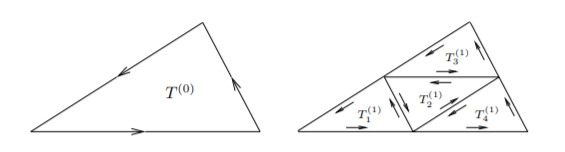
\includegraphics[height=8cm,width=16cm]{triangle.png} 
   \end{minipage}
\end{center}

Obviously, we may parametrize the boundaries of these triangles so that 
\begin{align*}
\int_{ \partial T^{(0)}}fdz= \sum_{n=1}^4 \int_{\partial T^{(1)}_n} fdz
\end{align*}
Taking absolute value on both side, we deduce 
\begin{align*}
  \abso{\int_{\partial  T^{(0)}}fdz }\leq 4 \abso{\int_{\partial  T^{(1)}_j}fdz}\text{ for some $j \in \set{1,2,3,4}$}
\end{align*}
Denote $T_j^{(1)}$ by $T^{(1)}$. Repeating this process, we obtain a decreasing sequence of triangles 
\begin{align*}
T^{(0)} \supseteq T^{(1)} \supseteq \cdots \supseteq T^{(n)} \supseteq \cdots 
\end{align*} 
with the property that
\begin{align}
\label{pe1}
\abso{\int_{\partial  T^{(0)}}fdz}\leq 4^n \abso{\int_{\partial T^{(n)}}fdz}
\end{align}
Let $d^{(n)}\text{ and }p^{(n)}$ denote the diameter and perimeter of $T^{(n)}$ for all $n\inz_0^+$. Some tedious effort shows that 
\begin{align}
\label{pe2}
d^{(n)}=2^{-n}d^{(0)}\text{ and }p^{(n)}=2^{-n}p^{(0)}
\end{align}
\myref{Theorem}{DSoC} implies 
\begin{align*}
\bigcap_{n\inn} T^{(n)}=\set{z_0}\text{ for some }z_0 \in D
\end{align*}
Because $f$ is holomorphic at  $z_0$, we may write $f:D\rightarrow \C$ by 
\begin{align*}
f(z)=f(z_0)+f'(z_0)(z-z_0)+o(z-z_0)(z-z_0)
\end{align*}
Clearly the first two terms have antiderivatives. Using \myref{Equation}{pe1} and \myref{Equation}{pe2}, we may now estimate 
\begin{align*}
 \abso{\int_{\partial T^{(0)}}f(z)dz}\leq  4^n\abso{\int_{\partial T^{(n)}} f(z)dz}&= 4^n\abso{\int_{\partial  T^{(n)}} o(z-z_0)(z-z_0)dz}\\
  &\leq 4^np^{(n)}d^{(n)}\max_{ z\in \partial T^{(n)}}\abso{o(z-z_0)}\\
  &= p^{(0)}d^{(0)} \max_{z \in \partial T^{(n)}} \abso{o(z-z_0)}\to 0\text{ as }n\to \infty
\end{align*}
\end{proof}
\begin{mdframed}
By $D\subseteq \C$ being \textbf{star-convex with center $z_*$}, we mean that for all $z \in D$, the contour $\gamma :[0,1]\rightarrow \C$ defined by 
\begin{align*}
\gamma (t)\triangleq z_*+t(z-z_*)
\end{align*}
satisfy $\gamma ([0,1])\subseteq D$. 
\end{mdframed}
\begin{theorem}
\textbf{(Existence of antiderivative on star-convex domain)} Suppose $D\subseteq \C$ is open and star-convex with centre  $z_*$. If $f:D\rightarrow \C$ is holomorphic, then $F:D\rightarrow \C$ defined by 
\begin{align*}
F(z)\triangleq \int_\gamma f(w)dw\text{ where }\gamma :[0,1]\rightarrow D\text{ is defined by }\gamma(t)\triangleq z_*+t(z-z_*)
\end{align*}
is an antiderivative of $f$. 
\end{theorem}
\begin{proof}
Fix $z_0 \in D$. Because $D$ is open, there exists some open ball $B_\epsilon (z_0)$ small enough to be contained by $D$. For all $z\in B_\epsilon (z_0)$, the closed triangle $T$ specified by the vertices $\set{z_*,z,z_0}$ is contained by $D$, since all $p\in  T$ lies in some line segment joining $z_*$ and $w$ where $w$ is some point that lies in the line segment joining $z$ and  $z_0$.  We then can apply \customref{CTft}{Cauchy's Integral Theorem for triangles} to have the estimate 
\begin{align*}
  \abso{\frac{F(z)-F(z_0)}{z-z_0}-f(z_0)}&= \abso{\frac{\int_\gamma [f(w)-f(z_0)]dw}{z-z_0}}\\
  &\leq \max_{w \in \gamma }\abso{f(w)-f(z_0)}\to 0\text{ as }z \to z_0
\end{align*}
where $\gamma$ is the line segment traveling from $z_0$ to  $z$.  
\end{proof}
\begin{mdframed}
At this point, it is appropriate for us to define \textbf{the winding number $w(\gamma ,z_0)$ of a contour $\gamma :[a,b]\rightarrow \C$ around some point $z_0\not\in \gamma $} by 
\begin{align*}
w(\gamma ,z_0)\triangleq  \frac{1}{2\pi  i}\int_{\gamma } \frac{1}{z-z_0}dz
\end{align*}
Immediately, we see that our definition satisfy our geometric intuition in the sense that the circle $\gamma :[0,2\pi  ]\rightarrow \C$ is defined by 
\begin{align*}
\gamma (t)\triangleq z_0 + e^{it}
\end{align*}
have winding number  
\begin{align*}
w(\gamma ,z_0)= \frac{1}{2\pi i}\int_0^{2\pi } e^{- it }ie^{it}dt= 1
\end{align*}
Moreover, we expect any closed contour $\gamma :[a,b]\rightarrow \C$ to have integer-valued winding number. This is true. Consider $f:[a,b]\rightarrow \C$ defined by 
\begin{align*}
f(t)\triangleq \frac{1}{2\pi  i}\int_a^t \frac{\gamma '(s)}{\gamma (s)-z_0}ds
\end{align*}
One may check by direct computation that 
\begin{align*}
\frac{d}{dt}e^{-2\pi  if (t)}(\gamma (t)-z_0)\equiv 0 
\end{align*}
It then follows from $\gamma $ being closed that 
\begin{align*}
e^{-2\pi  if(a)}=e^{-2\pi  if(b)}
\end{align*}
which implies 
\begin{align*}
w(\gamma ,z_0)=f(b)=f(a)+n=n\inz
\end{align*}
Given some contour $\gamma :[a,b]\rightarrow \C$, if we define $g:\C\setminus \gamma \rightarrow \C$ by 
\begin{align*}
g(z)\triangleq w(\gamma ,z)
\end{align*}
we see that $g$ is continuous, since if $z_0\not\in \gamma $, we may find $D_r(z_0)$ disjoint with $\gamma $ and obtain the estimate 
 \begin{align*}
\abso{w(\gamma ,z_0)-w(\gamma ,z_1)}&= \frac{1}{2\pi  }\abso{\int_\gamma \Big[ \frac{1}{z-z_0}-\frac{1}{z-z_1} \Big]dz} \\
&=\frac{1}{2\pi  }\abso{\int_{\gamma } \frac{z_1-z_0}{(z-z_0)(z-z_1)}dz} \\
&\leq \frac{L \abso{z_1-z_0}}{ r^2 \pi  }\text{ where }L\text{ is the length of }\gamma 
\end{align*}
as long as $\abso{z_0-z_1}<\frac{r}{2}$. The continuity of $g$ together with the fact that  $g$ can only be integer-valued implies that  $g$ is constant on any connected component of  $\C \setminus \gamma $. We may now finally state our version of \customref{CIT}{Cauchy Integral Theorem}. 
\end{mdframed}
\begin{theorem}
\label{CIT}
\textbf{(Cauchy Integral Theorem)} Suppose $D\subseteq \C$ is open and $f:D\rightarrow \C$ is holomorphic. If $\gamma :[a,b]\rightarrow \C$ is a closed contour lying in $D$ such that  $w(\gamma ,z)=0$ for all $z\not\in D$, then 
\begin{align*}
\int_\gamma  fdz=0 
\end{align*}
\end{theorem}
\begin{proof}
As Prof Frank remarked, the proof is omitted here for being too long and tricky. 
\end{proof}
\begin{theorem}
\label{CIF}
\textbf{(Cauchy Integral Formula)}  Let $U\subseteq \C$ be open, $D$ be an closed disk contained by  $U$, and $C$ be a closed contour running through the boundary of $D$ counterclockwise. If $f:U\rightarrow \C$ is holomorphic and $a\in D^\circ $, then 
\begin{align*}
f(a)= \frac{1}{2\pi  i}\int_C \frac{f(z)}{z-a}dz
\end{align*}
\end{theorem}
\begin{proof}
Fix $\epsilon $. Let $\delta$ satisfy 
\begin{align*}
\abso{z-a}\leq \delta \implies  \abso{f(z)-f(a)}\leq \epsilon 
\end{align*}
With a geometric argument using \customref{CIT}{Cauchy Integral Theorem}, one have 
\begin{align*}
\int_C \frac{f(z)}{z-a}dz=  \int_{\gamma  } \frac{f(z)}{z-a}dz
\end{align*}
where $\gamma :[0,2\pi ]\rightarrow D^\circ $ is defined by  
\begin{align*}
\gamma (t)\triangleq a+ \delta e^{it} 
\end{align*}
The proof then follows from the estimation 
\begin{align*}
  \abso{f(a)- \frac{1}{2\pi i}  \int_C \frac{f(z)}{z-a}dz}&= \abso{f(a)- \frac{1}{2\pi  i}\int_\gamma  \frac{f(z)}{z-a}dz} \\
                              &= \abso{f(a)- \frac{1}{2\pi  i}\int_0^{2\pi  } \frac{f(a+ \delta e^{it})}{\delta e^{it} } i\delta e^{i t} dt}  \\
                              &= \frac{1}{2\pi } \abso{\int_0^{2\pi  } f(a+ \delta e ^{it})- f(a)dt}\leq \epsilon 
\end{align*}
\end{proof}
\begin{theorem}
\label{Hfaa}
\textbf{(Holomorphic functions are analytic)} Let $U\subseteq \C$ be an open, $D$ be an closed disk contained by $U$ and centering $a$ with radius  $R$. Let $C$ be a closed contour running through the boundary of $D$ counterclockwise. If we define for all $n\geq 0$ 
\begin{align*}
c_n\triangleq  \frac{1}{2 \pi  i}\int_C \frac{f(z)}{(z-a)^{n+1}}dz
\end{align*}
then the power series 
\begin{align*}
  \sum_{n=0}^{\infty} c_n (z-a)^n
\end{align*}
agrees with $f$ on $D^{\circ }$. 
\end{theorem}
\begin{proof}
Let $z\in D^{\circ }$. By \customref{CIF}{Cauchy's Integral Formula}, we have 
\begin{align*}
f(z)&= \frac{1}{2\pi  i}\int_C \frac{f(w)}{w-z}dw \\
&=\frac{1}{2\pi  i}\int_C f(w)\Big[ \frac{1}{w-a} + \frac{z-a}{(w-a)^2}+ \cdots + \frac{(z-a)^m}{(w-a)^{m+1}} + \frac{(z-a)^{m+1}}{(w-a)^{m+1}(w-z)} \Big]dw \\
&=\sum_{n=0}^{m} c_n (z-a)^n + \frac{1}{2\pi  i}\int_C \frac{(z-a)^{m+1}}{(w-a)^{m+1}(w-z)}dw
\end{align*}
The proof then follows from noting  $\abso{\frac{z-a}{w-a}}<1$ and direct estimation of \myref{Equation}{LM}. 
\end{proof}
\begin{mdframed}
What follows from the fact  \customref{Hfaa}{holomorphic functions are analytic} and 
\customref{TT}{Taylor's Theorem for Power Series} is that if $f$ is holomorphic on some open disk  $D_{r+\epsilon }(a)$ and $C$ is the closed contour running through the boundary of  $D_r(a)$ counterclockwise, then we have a nice formula  
\begin{align*}
f^{(n)}(a)=  \frac{n!}{2\pi  i}\int_C \frac{f(z)}{(z-a)^{n+1}}dz
\end{align*}
which agrees with our \customref{CIF}{Cauchy integral Formula}.\\ 

In particular, we often encounter  complex function $f:\C\rightarrow \C$ that is \textbf{entire}, i.e., $f$ is holomorphic on the whole $\C$. \myref{Theorem}{Hfaa} states that for all $R>0$, if we let  $C$ be the closed contour running through the boundary of the open disk centering $0$ with radius  $R$  counterclockwise, then 
\begin{align*}
f=\sum_{n=0}^{\infty}c_{n,R} z^n \text{ on the open disk with radius }R
\end{align*}
for $c_{n,R}$ given in \myref{Theorem}{Hfaa}. Let $R_1< R_2$. Trivially, 
\begin{align*}
\sum_{n=0}^{\infty} c_{n,R_1}z^n=\sum_{n=0}^{\infty} c_{n,R_2}z^n\text{ on the open disk with radius }R_1
\end{align*}
It then follows from \customref{Identity Theorem}{Identity Theorem} that 
\begin{align*}
c_{n,R_1}=c_{n,R_2}\text{ for all }n
\end{align*}
Letting $R\to \infty$, we may now just write 
\begin{align*}
f(z)= \sum_{n=0}^{\infty}c_nz^n\text{ on }\C
\end{align*}
\end{mdframed}
\begin{theorem}
\label{LV}
\textbf{(Liouville's Theorem)} If entire $f:\C\rightarrow \C$ is bounded, then $f$ is constant. 
\end{theorem}
\begin{proof}
Write 
\begin{align*}
f(z)=\sum_{n=0}^{\infty}c_nz^n\text{ on }\C
\end{align*}
By \myref{Theorem}{Hfaa}, 
\begin{align*}
c_n= \frac{1}{2\pi i}\int_{C_r} \frac{f(z)}{z^{n+1}}dz
\end{align*}
where $C_r$ is the closed contour running through the boundary of the open disk centering  the origin with radius  $r$. Let $n\geq 1$, and let  $M$ be an upper bound of $\abso{f}$. The proof then following from letting $r \to \infty$ in the below estimation 
\begin{align*}
\abso{c_n}= \frac{1}{2\pi } \cdot (2\pi r) \cdot \max_{C_r} \abso{\frac{f(z)}{z^{n+1}}} \leq \frac{M}{r^n}
\end{align*}
\end{proof}
\section{Residue Formula}
\begin{abstract}

\end{abstract}
\begin{mdframed}
Before we begin developing this section, we first give the following remark. Let  
\begin{align*}
0<R_1 <r_1<r_2<R_2 < \infty
\end{align*}
Let $C_1,C_2$ respectively be closed contours running through the boundary of $D_{r_1}(0),D_{r_2}(0)$. If $f$ is holomorphic on on $R_1 < \abso{z}<R_2$, then 
\begin{align*}
\int_{C_1} f(z)dz= \int_{C_2}f(z)dz
\end{align*}
by a simple geometric argument. Therefore, we may give the next Theorem a well-defined statement. 
\end{mdframed}
\begin{theorem}
\label{LTC}
\textbf{(Laurent's Theorem)} Suppose
\begin{align*}
0\leq R_1 <r< R_2 \leq \infty
\end{align*}
$C_r$ is a closed contour running through the circle centering $z_0$ with radius $r$ counterclockwise, and $f$ is holomorphic on the annulus $R_1 < \abso{z-z_0} < R_2$. If we define 
\begin{align*}
c_n\triangleq  \frac{1}{2\pi  i} \int_{C_r} \frac{f(z)}{(z-z_0)^{n+1}}dz\text{ for all }n\inz
\end{align*}
Then $\sum_{n\geq 0} c_nh^n$ converge for $\abso{h}<R_2$, $\sum_{n<0} c_nh^{n}$ converge for $\abso{h}>R_1$ and 
\begin{align*}
f(z_0+h)= \sum_{n\inz} c_nh^n\text{ on the annulus }R_1 < \abso{h}< R_2
\end{align*}
\end{theorem}
\begin{proof}
Fix some  $h\inc$ such that $R_1 < \abso{h}<R_2$. Let $r_1,r_2$ satisfy 
 \begin{align*}
R_1 < r_1 < \abso{h}< r_2 < R_2
\end{align*}
And let $C_{r_1},C_{r_2}$ respectively be closed contours running through the circle centering $z_0$ with radius  $r_1,r_2$ counterclockwise. We first show that 
\begin{align*}
  \vi{f(z_0+h)= \frac{1}{2\pi  i}\int_{C_{r_1}} \frac{f(z)}{z-(z_0+h)}dz- \frac{1}{2\pi i}\int _{C_{r_2}} \frac{f(z)}{z-(z_0+h)}dz}
\end{align*}
\end{proof}
\begin{mdframed}
With \customref{LTC}{Laurent's Theorem}, given holomorphic $f:D_\epsilon (z_0)\setminus \set{z_0}\rightarrow \C$, we may write 
\begin{align*}
f(z)= \sum_{n\inz} c_n (z-z_0)^n\text{ for } 0<\abso{z-z_0}< \epsilon 
\end{align*}
If $c_n=0$ for all $n<0$, obviously we may define  $f(z_0)\triangleq c_0$, so that $f$ is still holomorphic after such extension. If this is the case, we say $f$ has a  \textbf{removable singularity at $z_0$}.     
\end{mdframed}
\begin{theorem}
\label{RoRS}
\textbf{(Riemann's removable singularity Theorem)} Given holomorphic $f:D_\epsilon (z_0)\setminus \set{z_0}\rightarrow \C$ 
\begin{align*}
z_0\text{ is a removable singularity of $f$ }\iff f\text{ is bounded on some }D_\delta (z_0)\setminus \set{z_0}
\end{align*}
\end{theorem}
\begin{proof}
From left to right is clear. Suppose $f$ is bounded by $M$ on $D_\delta(z_0)\setminus \set{z_0}$. Because 
\begin{align*}
c_n=\frac{1}{2\pi  i}\int_{C_r}f(z)(z-z_0)^{-n-1}dz
\end{align*}
We may estimate 
\begin{align*}
  \abso{c_n}\leq \frac{1}{2\pi }(2\pi r )( M r^{-n-1})= Mr^{-n}
\end{align*}
The proof then follows from letting $n<0$ and $r \to 0$. 
\end{proof}
\begin{mdframed}
If for some $m<0$, we have  
 \begin{align*}
c_m \neq 0\text{ and }c_n=0\text{ for all }n\leq m
\end{align*}
then we say $f$ has a  \textbf{pole of order $m$ at  $z_0$}. If a pole is of order $1$, we say such pole is a  \textbf{simple pole}.  
\end{mdframed}
\begin{theorem}
\textbf{(Recognition of Pole)} Given holomorphic $f:D_\epsilon (z_0)\setminus \set{z_0}\rightarrow \C$ 
\begin{align*}
f\text{ has a pole of order }m\text{ at }z_0\iff \lim_{z\to z_0}(z-z_0)^mf(z)\inc^*
\end{align*}
\end{theorem}
\begin{proof}
From left to right is clear. From right to left, define $g:D_\epsilon (z_0)\setminus \set{z_0}\rightarrow \C$ by 
\begin{align*}
g(z)\triangleq (z-z_0)^m f(z)
\end{align*}
From premise, we may deduce $g$ is bounded on some  $D_\delta(z_0)\setminus \set{z_0}$. Therefore, by \myref{Theorem}{RoRS}, $g$ has a removable singularity at $z_0$. Thus, we may write 
 \begin{align*}
g(z)=\sum_{n=0}^{\infty}a_n z^n
\end{align*}
where $a_0\neq 0$ by premise. The proof then follows from writing $f$ in terms of $a_n$.  
\end{proof}
\begin{mdframed}
Writing holomorphic $f:D_\epsilon (z_0)\setminus \set{z_0}\rightarrow \C$ in terms of Laurent Series  
\begin{align*}
f(z)= \sum_{n\inz} c_n (z-z_0)^n 
\end{align*}
We define the \textbf{residue of $f$ at  $z_0$} to be 
\begin{align*}
\operatorname{Res}(f,z_0)\triangleq c_{-1}
\end{align*}
If there are infinitely many $n<0$ such that $c_n\neq 0$, we say $f$ has a \textbf{essential singularity} at $z_0$. Obviously, if  $f$ has a removable singularity at  $z_0$, then the residue of  $f$ at $z_0$ is  $0$. Immediately, from direct computation with Laurent expansion of $f:D_\epsilon (z_0)\setminus \set{z_0}\rightarrow \C$, we may conclude the following easy ways to compute residue for relatively simple function. 
\end{mdframed}
\begin{theorem}
\textbf{(Calculation of Residue)} If holomorphic $p,q:D_\epsilon (z_0)\rightarrow \C$ satisfies 
\begin{align*}
p(z_0)\neq 0\text{ and }q(z_0)=0,q'(z_0)\neq 0 
\end{align*}
Then $f=\frac{p}{q}$ has a simple pole at $z_0$ and 
 \begin{align*}
\operatorname{Res}(f,z_0)= \frac{p(z_0)}{q'(z_0)}
\end{align*}
If $f:D_\epsilon (z_0)\setminus \set{z_0}\rightarrow \C$ has a pole of order $m$ at  $z_0$,  then 
 \begin{align*}
\operatorname{Res}(f,z_0)=  \lim_{z\to z_0} \frac{1}{(m-1)!} \Big( \frac{d}{dz} \Big)^{m-1} (z-z_0)^m f(z)
\end{align*}
\end{theorem}
\begin{theorem}
\label{CRT}
\textbf{(Cauchy's Residue Theorem)} Suppose that $f$ is holomorphic in an open set containing a positively oriented  Jordan curve $\gamma $ and its interior, except for poles at the points $z_1,\dots ,z_N$ inside $\gamma $. Then 
\begin{align*}
\int_{\gamma }f(z)dz = 2\pi  i\sum_{n=1}^N \operatorname{Res} (f,z_n)
\end{align*}
\end{theorem}
\begin{mdframed}
  Using \customref{CRT}{the residue theorem}, we may compute the following integral that will definitely exists in context of Fourier analysis.   
\end{mdframed}
\begin{Example}{\textbf{(Poisson Kernel)}}{}
\begin{align*}
  \int_0^{\pi } \frac{\log x}{1+x^2}dx
\end{align*}
\end{Example}
\begin{mdframed}
Let $D \subseteq \C$ be open connected, $f:D\rightarrow \C$ be holomorphic. Suppose $f$ does not vanish identically on  $D$.  \customref{Identity Theorem}{Identity Theorem} tell us that the set of \textbf{zeros}
\begin{align*}
Z\triangleq \set{z\in D: f(z)=0}
\end{align*}
must have no limit point in $D$. Therefore, for each zero $z_0 \in Z$, when we write locally 
\begin{align*}
  f(z)= \sum_{n=0}^{\infty} c_n(z-z_0)^n
\end{align*}
there exists some smallest $n\geq 1$ such that $c_n \neq 0$. We then say $f$ has a  \textbf{zero of order $n$ at $z_0$}, and if  $n=1$, we say this zero is  \textbf{simple}. \\

Let $z_0\inc$. Given some holomorphic $f:D_\epsilon (z_0)\setminus \set{z_0}\rightarrow \C$, we say $f$ has a \textbf{removable singularity at $z_0$} if we may define $f(z_0)$ to be some complex number so that $f:D_\epsilon (z_0)\rightarrow \C$ is holomorphic. Suppose $f:D_\epsilon (z_0)\setminus \set{z_0}\rightarrow \C^*$. We say $f$ has a  \textbf{pole of order $n$ at $z_0$} if the function $g:D_\epsilon (z_0)\rightarrow \C$ defined by 
\begin{align*}
g(z)\triangleq \begin{cases}
  \frac{1}{f(z)}& \text{ if $z\neq z_0$ }\\
  0& \text{ if $z=z_0$ }
\end{cases}
\end{align*}
is holomorphic with the order $n$ at zero  $z_0$. Obviously, there exists an unique holomorphic $h:D_\epsilon (z_0)\rightarrow \C$ such that 
\begin{align*}
g(z)= (z-z_0)^n h(z)
\end{align*}
It is clear that $h$ does not vanish on  $D_\epsilon (z_0)$. Therefore, we may write 
\begin{align*}
G(z)= \frac{1}{h(z)}
\end{align*}
so that $G:D_\epsilon (z_0)\rightarrow \C$ is holomorphic and write 
\begin{align*}
f(z)= \frac{G(z)}{(z-z_0)^n}=\sum_{k=-n}^{\infty}a_k (z-z_0)^k
\end{align*}
We then call 
\begin{align*}
\sum_{k=-n}^{-1}a_k(z-z_0)^k
\end{align*}
the \textbf{principal part of $f$ at the pole $z_0$} and 
\begin{align*}
\operatorname{Res}_{z_0}f\triangleq a_{-1}
\end{align*}
the \textbf{residue of $f$ at the pole  $z_0$}. It is clear from the Laurent expansion of $f$ and direct computation that   
\begin{align*}
\operatorname{Res}_{z_0}f=
\end{align*}
\end{mdframed}
\end{document}
